\documentclass[fleqn]{report}

\usepackage[utf8]{inputenc}
\usepackage{cite}

\usepackage{amsfonts}
\usepackage{amsmath}
\usepackage{amssymb}
\usepackage{float}

\usepackage{hyperref}

\usepackage{syntax}
\setlength{\grammarparsep}{0cm}

\usepackage{zed-csp}
\usepackage{lipsum}
\usepackage{xspace}
\usepackage[margin=1.55in]{geometry} %page size

\usepackage{tikz}
\usetikzlibrary{positioning}

\usepackage{listings}
\lstdefinelanguage{sal}{
  keywords = {send, become, let, new, in, to, if, then, else, case, def, end,
    case, of, ||}
}


\lstdefinestyle{simple}{
  numbers=left,
  basewidth=0.5em
}

\newcommand{\SAL}{\textbf{SAL}\xspace}
\newcommand{\CSP}{\textbf{CSP}\xspace}
\newcommand{\CSPm}{\textbf{CSPm}\xspace}


\begin{document}

\begin{titlepage}
%\begin{adjustwidth*}{-1cm}{-2.7cm}
\centering
\vspace*{0.5 cm}
        \includegraphics[width=3.0 cm]{img/logo.png}\\[1.0 cm]
        \textsc{\LARGE Universidad Nacional de Rosario}\\[0.5 cm]
	\textsc{\large Departamento de Ciencias de la Computaci\'{o}n}\\[2.5 cm]

	\rule{\linewidth}{0.3 mm} \\[0.4 cm]
	{ \huge \bfseries Un modelo semántico para Actores basado en CSP }\\
	\rule{\linewidth}{0.3 mm} \\[0.5 cm]
	\textsc{\Large Tesina de grado}\\[2.5 cm]
	
	\begin{minipage}{0.4\textwidth}
	\begin{flushleft} \large
	  \emph{Autor:}\\
	  José Luis Diaz  \\
	\end{flushleft}
	\end{minipage}~
	\begin{minipage}{0.4\textwidth}
        \begin{flushright} \large
	  \emph{Directores:} \\
	  Maximiliano Cristía \\
	  Hernán Ponce de León \\
	\end{flushright}        
	\end{minipage}\\[1.5 cm]
        \today

%\end{adjustwidth*}
\end{titlepage}

\tableofcontents

\chapter{Introducción}

\section{Motivación}

Debido al incremento de la cantidad de núcleos por microprocesador, las aplicaciones hacen un uso más frecuente de la concurrencia. Una forma de programar este tipo de aplicaciones es utilizando el modelo tradicional de concurrencia que se basa en multi-hilos, variables compartidas, locks, etc. Este trabajo propone estudiar un enfoque diferente: el modelo de actores utilizado en la industria, particularmente en lenguajes como Erlang\cite{Cesarini:2009:EP:1717841, Armstrong:1996:CPE:229883} y Scala\cite{scala-overview-tech-report} con la librería Akka\cite{Wyatt:2013:AC:2663429}. 

El objetivo de este trabajo es comprender el modelo de actores y su semántica. Con este fin, luego de explorar las características del modelo de actores, se introduce un lenguaje simple de actores llamado \SAL cuya semántica se formalizara en \CSP. Con este modelo se realizan algunas pruebas utilizando la herramienta \FDR, tales como revisión del árbol de ejecución y verificación de refinamiento utilizando el modelo de traza. Se presentan varios ejemplos con el fin de ayudar al lector a comprender el paradigma de programación concurrente basado en actores.

La diferencia entre ambos modelos se puede notar mediante el problema del jardín ornamental. El enunciado del problema es el siguiente: supongamos que tenemos dos entradas a un parque y se requiere saber cuanta gente ingresa. Para eso se instala un molinete en cada entrada. Se utiliza una computadora para registrar la información de ingreso.

Siguiendo el modelo tradicional de concurrencia, se incluiría una variable global que guarde la cantidad de visitantes y dos hilos representando los molinetes que incrementan esta variable. Sin ningún tipo de protección en la región crítica planteada por la actualización de la variable global podrían perderse incrementos, ya que cada hilo carga localmente el valor de la variable global, efectúa un incremento y finalmente guarda el valor en la variable global. 

El mismo problema se puede escribir utilizando el modelo de actores, que tiene como único mecanismo de comunicación entre entidades el paso de mensajes. En este caso, el problema puede ser representado utilizando un actor que realiza la tarea de contador. Este incrementará su valor cuando reciba un mensaje \emph{inc}. Otros dos actores emitirán los mensajes \emph{inc} (los molinetes). En este caso el problema de la pérdida de la actualización no ocurre.

El modelo de actores fue originalmente propuesto por C. Heweeit\cite{Wyatt:2013:AC:2663429}. Es un enfoque diferente a cómo estructurar programas concurrentes. Según este modelo un actor es una entidad computacional que puede:

\begin{itemize}
\item Enviar y recibir un número finito de mensajes a otros actores.
\item Crear un número finito de actores.
\item Designar un nuevo comportamiento a ser usado cuando se reciba el próximo mensaje.
\end{itemize}

Como señala Rob Pike en su charla titulada ``Concurrencia no es paralelismo'' \cite{rpike13:cnp}, muchas veces se pasa por alto la diferencia conceptual entre la concurrencia y el paralelismo. En programación, la concurrencia es la composición de los procesos independientemente de la ejecución, mientras que el paralelismo es la ejecución simultánea de cálculos (posiblemente relacionados). El modelo de actores, mejora sustancialmente la composición.

\section{Objetivo}
El objetivo de este trabajo es comprender el modelo de actores y su semántica. Una buena herramienta para asistir a este proceso es utilizar métodos formales. Se propone modelar la semántica del modelo de actores en \CSP y efectuar algunas pruebas utilizando la herramienta \FDR\cite{fdr}.

\subsubsection*{CSP}

\textit{Communicating Sequential Processes} (\CSP), fue propuesto por primera vez por C.A.R Hoare\cite{Hoare:1978:CSP:359576.359585}. Es un lenguaje para la especificación y verificación del comportamiento concurrente de sistemas. Como su nombre lo indica, \CSP permite la descripción de sistemas en términos de componentes que operan de forma independiente e interactúan entre sí únicamente a través de eventos sincrónicos. Las relaciones entre los diferentes procesos y la forma en que cada proceso se comunica con su entorno, se describen utilizando un álgebra de procesos.

\subsubsection*{FDR}

Es una herramienta para el análisis de los modelos escritos en \CSP. El lenguaje de entrada de \FDR, \CSPm, combina los operadores de \CSP con un lenguaje de programación funcional. \FDR originalmente fue escrito en 1991 por Formal Systems (Europe) Ltd, que también lanzo la versión 2 a mediados de la década de 1990. La versión actual de la herramienta esta disponible gracias a la Universidad de Oxford. Se puede utilizar para fines académicos si necesidad de una licencia, siendo sí necesaria para fines comerciales.

Si bien tanto \CSP como el modelo de actores apuntan al problema de la concurrencia, no lo modelos tienen entidades concurrentes que intercambian eventos o mensajes. Sin embargo, los dos modelos toman algunas decisiones fundamentalmente diferentes con respecto a las primitivas que proporcionan:

\begin{itemize}
\item Los procesos de \CSP son anónimos, mientras que los actores tienen identidades.
\item En \CSP los procesos involucrados en el envío y la recepción de un evento deben sincronizar. Es decir, el remitente no puede transmitir un evento hasta que el receptor está dispuesto a aceptarlo. Por el contrario, en los sistemas de actores, el paso de eventos es fundamentalmente asíncrono, es decir, la transmisión y la recepción de eventos no tienen que suceder al mismo instante.
\item \CSP utiliza canales explícitos para el paso de datos, mientras que los sistemas de actores transmiten datos a los actores de destino mediante la dirección de su buzón.
\end{itemize}

Estos enfoques pueden ser considerados duales el uno al otro, en el sentido de que los sistemas basados en \emph{sincronización} pueden utilizarse para construir comunicaciones que se comporten como sistemas de mensajería asíncrona, mientras que los sistemas asíncronos se pueden utilizar para construir las comunicaciones sincrónicas utilizando algún protocolo que permita el encuentro entre los procesos. Lo mismo ocurre con los canales.

\section{Trabajos Relacionados}

En su tesis doctoral Agha\cite{Agha:1986:AMC:7929} define en detalle el modelo de actores. También define dos lenguajes \SAL y \ACT. Da una semántica denotacional a \SAL. Este trabajo sigue de cerca este lenguaje, y construye una semántica en \CSP.

En el trabajo \textit{An Algebraic Theory of Actors and its Application to a Simple Object-Based Language}\cite{apicalculus}, Gul Agha y Prasanna Thati definen un modelo algebraico del modelo de actores, y sobre el final le dan semántica a \SAL.

En su tesis doctoral Clinger\cite{Clinger:1981} presenta una teoría para una clase de lenguajes no deterministas que incluyen paralelismo, enfocado específicamente en el modelo de actores.

Se puede ver en el trabajo \textit{An algebra of actors}\cite{algebraActors}, que los autores definen un algebra de procesos y proveen una semántica operacional basada en un sistema de transición etiquetado.

En el trabajo \textit{Formalising Actors in Linear Logic}\cite{actorLiniarLogic}, los autores definen un formalismo basado en actores en términos la deducción en lógica lineal.

Otro lenguaje que implementa el modelo de actores es Pony\cite{ponylang}, utiliza memoria compartida para evitar duplicación de memoria cuando se envían mensajes. Esto puede llevar a una o varias \textit{condiciónes de carreras}. Para evitar este tipo de problemas, tiene definido un sistema de permisos, con una prueba formal\cite{Clebsch:2015:DCS:2824815.2824816}. Este sistema de permisos leer, escribir y atravesar referencias únicas evitando este problema.

\section{Organización de este trabajo}

En el capítulo 2 se introduce el modelo de actores y se describe la sintaxis de \SAL. En el capítulo 3 se presentan los conceptos necesarios de \CSP y \CSPm, que serán luego utilizados en el siguiente capítulo. El capítulo 4 construye un modelo de actores utilizando \CSP donde, se presentan varios ejemplos. Se muestra una semántica de \SAL en \CSP. Se termina mostrando como este modelo puede ser utilizado en la herramienta \FDR. Finalmente, el capítulo 5 presenta algunas conclusiones del trabajo y los posibles trabajos futuros.
 % Introducción

\chapter{Sistema de actores}

\newcommand{\COMUNICACIONES}{\mathcal{K}}
\newcommand{\COMUNICACIONESSUB}{\mathsf{K}}

\newcommand{\COMUNICACION}{\bar{k}}
\newcommand{\BUZONES}{\mathcal{B}}
\newcommand{\BUZONESSUB}{\mathsf{B}}
\newcommand{\BUZON}{\beta}
\newcommand{\MENSAJES}{\mathcal{M}}
\newcommand{\MENSAJE}{m}

\newcommand{\ACTOR}{\alpha}
\newcommand{\COMPORTAMIENTOS}{\mathcal{C}}
\newcommand{\COMPORTAMIENTOSSUB}{\mathsf{C}}

\newcommand{\COMPORTAMIENTO}{c}
\newcommand{\COMNOPROC}{\kappa}

En este capítulo se explica cómo funciona la estructura computacional en el modelo de actores. En la primera sección se introduce el funcionamiento de las comunicaciones y el comportamiento de los actores. En la segunda sección se define la sintaxis de un lenguaje mínimo de actores, para terminar con algunos ejemplos utilizando este lenguaje.

\section{Describiendo un sistema de actores}
Un sistema de actores consiste de configuraciones. Una configuración viene dada por una colección de actores concurrentes y una colección de comunicaciones en tránsito. Cada actor tiene un nombre único y un comportamiento. Se comunica con otros actores a través de mensajes asíncronos. Los actores son reactivos, es decir, ejecutan solo en respuesta a los mensajes recibidos. El comportamiento de un actor es determinista, ya que la respuesta está determinada por el contenido del mensaje que procesa. 

\subsection{Comunicaciones}

Se puede decir que las comunicaciones que no son fueron procesadas son quienes mueven los cálculos en un sistema de actores. Las comunicaciones vienen representados por el par:

\begin{enumerate}
\item \textit{destino}, la dirección de buzón a la que será entregada la comunicación. 
\item \textit{mensaje}, básicamente la información que estará disponible al actor que procesará la comunicación.
\end{enumerate}

Un \textit{mensaje} es una lista de valores. Estos valores pueden ser: direcciones de buzón, enteros, cadenas de caracteres, etc. 

El \textit{destino} debe ser una dirección de buzón válida, es decir, un actor antes de enviarle una comunicación a otro actor debe tener la dirección de buzón destino, y esta debe ser válida. Existen tres formas en la cual un actor $\ACTOR$, al aceptar una comunicación $\COMUNICACION$, puede conocer la dirección de buzón de otro actor:

\begin{itemize}
 \item El \textit{destino} era conocido por el actor $\ACTOR$, antes de aceptar la comunicación.
 \item El \textit{destino} estaba incluido como parte de la comunicación $\COMUNICACION$.
 \item El \textit{destino} es una dirección de buzón creada como resultado de aceptar la comunicación $\COMUNICACION$.
\end{itemize}

Es probable que más de un actor al mismo tiempo quiera enviar una comunicación a un buzón. Para esto es necesario alguna estructura intermedia que guarde todas las comunicaciones creadas y que aún no fueron procesadas. Esta estructura tiene que tener la capacidad para guardar todas las comunicaciones hasta ser procesadas por el actor destino. 

%En realidad Agha\ [chap.~3,p.~35]\cite{Agha:1986:AMC:7929} lo define como una 3-tupla incluye un \textit{tag} para diferenciar una tarea de la otra en el sistema. Define que un \textit{tag} puede tener una representación arbitraria. Como los \textit{tag} son únicos en todo el sistema, hace uso de esta propiedad para construir la direcciones de buzón de los nuevos actores creados esto puede verse en \cite[chap.~5,p.~104]{Agha:1986:AMC:7929}. 

% En el modelo que se presentará esto no es necesario.
% Otro de los argumentos sobre incluir este \textit{tag} esta relacionado con tener trazabilidad, como diferenciar dos tareas que tienen el mismo destino y la misma comunicación. En este trabajo podriamos incluir un numero aleatorio para permitir tener esta trazabilidad si quisieramos diferenciar estas dos tareas \textit{destino} y la misma \textit{comunicación}, pero se decidió dejarlo fuera.

\subsection{Actores}

Toda computación en el modelo de actores es resultado de procesar comunicaciones. Un actor acepta un mensaje cuando este es procesado. Un actor sólo puede procesar comunicaciones que están dirigidas a su dirección de buzón. Como resultado de aceptar una comunicación, un actor puede: crear nuevas comunicaciones, crear nuevos actores y debe definir su comportamiento de reemplazo.

%Para un actor, el orden de llegada de las comunicaciones enviadas a ese actor debe ser lineal. Esto quiere decir el buzón debería tener algún mecanismo de \textit{buffer} para las comunicaciones que lleguen casi al mismo tiempo. 

Un actor puede describirse especificando:

\begin{itemize}
 \item Su dirección de buzón, a la que le corresponde un \textit{buzón} lo suficientemente grande para almacenar las comunicaciones aún no procesadas.
 \item Su \textit{comportamiento}, que es una función que tiene la comunicación que está siendo procesada como entrada y como salida nuevos actores, nuevas comunicaciones y su nuevo comportamiento de reemplazo.
\end{itemize}

Podemos pensar que un actor es un \textit{buzón} donde llegan todas las comunicaciones, y un proceso que ejecutará su comportamiento. Este proceso apunta a una comunicación particular de este \textit{buzón}. 

% \begin{figure}[H]
% \begin{tikzpicture}
% 
% \draw (0,0) -- (7,0);
% \draw (0,1) -- (7,1);
% 
% \draw (0,0) -- (0,1);
% \draw (0.5,0) -- (0.5,1);
% \draw (1,0) -- (1,1);
% 
% \draw (5,0) -- (5,1);
% \draw (5.5,0) -- (5.5,1);
% 
% \node at (0.9,1.2) {$1\quad2\quad\ldots$};
% 
% \node at (5.25,1.2) {$n$};
% 
% \node at (7.8,0.5) {comunicaciones sin procesar};
% 
% \node at (6.4,-1.4) {proceso};
% 
% \draw[->] (5.25,-1) -- (5.25,0);
% \node at (5.25,-1.4) [circle,draw] (x) {$X$};

% \end{tikzpicture}
% \caption{Representación de un actor. El proceso tiene la información de su comportamiento. Acepta la comunicación actual y no puede procesar ningún otra comunicación.}
% \label{fig:mailqueue}
% \end{figure}

Cuando el proceso $X_n$ acepta la $(n)-\acute{e}sima$ comunicación, eventualmente crea el proceso $X_{n+1}$ el cual ejecutará el comportamiento de reemplazo definido por $X_n$. Este nuevo proceso apunta a la siguiente comunicación en el buzón en donde estará guardada la comunicación $(n+1)-\acute{e}sima$. Esto puede verse en la figura \ref{fig:actortransition}

\begin{figure}[H]
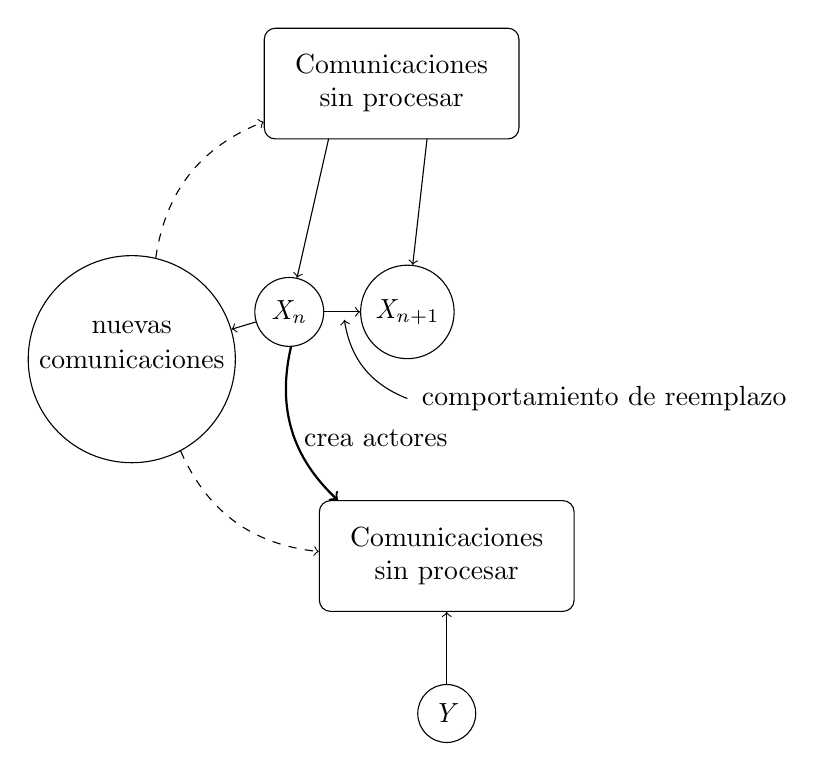
\begin{tikzpicture}
\tikzstyle{block} = [rectangle, draw, text width=3cm, text centered, rounded corners, minimum height=4em,font=\normalsize]

\node at (4,-2.4) [circle,draw] (XN) {$X_n$};
\draw[<-] (XN) -- (4.5,-.2);

\node at (5.5,-2.4) [circle,draw] (XN1) {$X_{n+1}$};
\draw[<-] (XN1) -- (5.75,-.2);

\draw[->] (XN) -- (XN1);

\node at (2,-2.6) {nuevas};
\node at (2,-3) [circle,draw] (K) {comunicaciones};



\draw[->] (XN) -- (K);

\node at (8,-3.5) {comportamiento de reemplazo};

\draw[->] (5.5,-3.5) to[bend left] (4.7,-2.5); 
\node[block, draw] (C1) at (5.3,0.5) {Comunicaciones sin procesar};

\node[block, draw] (C2) at (6,-5.5) {Comunicaciones sin procesar};

\draw[->, thick] (XN) to[bend right] (C2);
\node at (5.1,-4) {crea actores};

\node[below of=C2,yshift=-1cm, circle,draw] (Y) {$Y$};

\draw[->] (Y) -- (C2.south);

\draw[->, dashed] (K) to[bend left] (C1);
\draw[->, dashed] (K) to[bend right] (C2);


\end{tikzpicture}
\caption{Una transición entre dos comportamientos}
\label{fig:actortransition}
\end{figure}
Los dos procesos $X_n$ y $X_{n+1}$ no interfieren entre sí, pero la creación de $X_{n+1}$ depende de que $X_{n}$ haya definido su comportamiento de reemplazo. $X_n$ solo procesa la $(n)-\acute{e}sima$ comunicación. Exceptuando el caso en el cual se envíe una comunicación a sí mismo, en este caso indirectamente estaría interfiriendo. Cada uno de estos procesos crean sus propias tareas, sus propios actores como esta definido en sus comportamientos. Antes que el proceso $X_n$ cree el proceso $X_{n+1}$, $X_n$ podría haber creado otros actores u otros trabajos. Es posible incluso, que $X_n$ esté creando actores o trabajos al mismo tiempo que lo está haciendo $X_{n+1}$. Es importante notar que $X_n$ no recibirá ninguna otra comunicación, ni tampoco especificará ningún otro comportamiento de reemplazo.
% Si definimos que la creación de un actor, la creación de una tarea o especificar el comportamiento de reemplazo son eventos. El orden en que se generan estos eventos debido a que se acepto una comunicación define un orden parcial. El reemplazo de los procesos definen un orden total entre ellos. 

Esto parecería definir algún tipo de orden con respecto a cómo se van a procesar los mensajes. Sin embargo, el trabajo de Agha\cite{Agha:1986:AMC:7929} no se define ningún orden específico sobre el procesamiento de comunicaciones. La única garantía que el modelo provee es sobre las comunicaciones, está relacionada con el eventual proceso de los mensajes. Tanto la implementación de Erlang\cite{Cesarini:2009:EP:1717841} como la implementación de Akka\cite{Wyatt:2013:AC:2663429}, entregarán al menos una vez la comunicación a un actor, pero no garantizan la entrega.

%Alguna implementación puede esperar que el proceso anterior termine, para construir el nuevo y eliminar el viejo. Sin embargo, retrasar el reemplazo hasta que el proceso pueda ser reemplazado no es un requisito. Si hay suficientes recursos disponibles, la computación en un sistema de actores se puede acelerar simplemente aceptando la próxima comunicación ni bien su comportamiento de reemplazo este establecido.

\begin{figure}[H]
\centering

\tikzstyle{circulo}=[circle,draw=black, fill=black, inner sep=0pt,minimum size=3pt]
\tikzstyle{new}=[-latex, draw, dashed]
\tikzstyle{msg}=[-latex, draw]

\begin{subfigure}{.5\textwidth}
\centering
\begin{tikzpicture}[node distance=2cm]

\node[] (A) {$Actor_1$};
\node[circulo, below of=A] (A1) {};
\node[circulo, below of=A, yshift=0.3cm] (A11) {};

\node[below of=A1] (A2) {};
\draw (A) -- (A2);

\node[below of=A, right of=A, yshift=1cm] (B) {$Actor_2$};
\node[circulo, below of=A, right of=A] (B1) {};

\node[below of=B1] (B2) {};
\draw (B1) -- (B2);


%\path[msg] (-1/2,-1/2) to [bend right] node[font=\small, left] {$[42]$}  (A1) ;

%\path[new] (A1) to [bend left] node[font=\small, above] {$[7]$} (B1) ;
%\path[new] (A1) to [bend right] node[font=\small, below, pos=0.6] {$[8,9]$} (C1) ;

\path[msg] (-1/2,-1/2) to [bend right] (A11) ;

\path[new] (A1) to [bend left] (B1) ;

\end{tikzpicture}

\caption{  }
\label{fig:actores:crecion:a}
\end{subfigure}%
\begin{subfigure}{.5\textwidth}

\centering
\begin{tikzpicture}[node distance=2cm]

\tikzstyle{circulo}=[circle,draw=black, fill=black, inner sep=0pt,minimum size=3pt]

\node[] (A) {$Actor_1$};
\node[circulo, below of=A] (A1) {};
\node[circulo, below of=A, yshift=0.3cm] (A11) {};
\node[below of=A1] (A2) {};
\draw (A) -- (A2);

\node[right of=A] (B) {$Actor_2$};
\node[circulo, below of=A, right of=A] (B1) {};
\node[circulo, below of=A, right of=A, yshift=-0.3cm] (B11) {};

\node[below of=B1] (B2) {};
\draw (B) -- (B2);

\node[right of=B1, yshift=1cm] (C) {$Actor_3$};
\node[circulo, right of=B1, yshift=-0.3cm] (C1) {};

\node[below of=C1, yshift=0.3cm] (C2) {};
\draw (C1) -- (C2);

%\path[msg] (-1/2,-1/2) to [bend right] node[font=\small, left] {$[43]$}  (A1) ;

%\path[msg] (A1) to [bend left] node[font=\small, above] {$[1,2]$} (B1) ;
%\path[new] (B1) to [bend left] node[font=\small, above] {$[3,4]$} (C1) ;

\path[msg] (-1/2,-1/2) to [bend right] (A11) ;
\path[msg] (A1) to [bend left] (B1) ;
\path[new] (B11) to [bend left] (C1) ;

\end{tikzpicture}

\caption{}
\label{fig:actores:crecion:b}
\end{subfigure}

\caption{Las lineas verticales indican el paso del tiempo, las de punto indican creación de actores y las otras flechas envío de mensaje.}
\label{fig:actores:crecion}
\end{figure}

% Como se puede ver en la figura \ref{fig:actores:crecion} \subref{fig:actores:crecion:a}, el actor $Actor_1$ recibe una comunicación. Al procesar esta comunicación, crea el actor $Actor_2$. En la figura \ref{fig:actores:crecion} \subref{fig:actores:crecion:b} se puede ver un ejemplo similar donde $Actor_1$ recibe una comunicación, como resultado envía una comunicación a $Actor_2$ y este último crea $Actor_3$.

\subsection{Dinámica del modelo de actores}

Las comunicaciones están definidas por el par buzón destino y mensaje, de la siguiente forma:
\begin{align}\label{eq:comunicaciones}
\COMUNICACIONES = \BUZONES \times \MENSAJES
\end{align}
donde $\BUZONES$ es el conjunto de las direcciones buzón, $\MENSAJES$ es el conjunto de los mensajes. 

La definición de los comportamiento viene dada de la siguiente forma:
\begin{align}\label{eq:comportamientos}
\COMPORTAMIENTOS : \COMUNICACIONES \rightarrow ( \{ \COMUNICACION_1, \COMUNICACION_2, \ldots, \COMUNICACION_m \}, \{ \ACTOR_1, \ACTOR_2, \ldots, \ACTOR_n \}, \COMPORTAMIENTO )
\end{align}
donde $\{ \COMUNICACION_1, \COMUNICACION_2, \ldots, \COMUNICACION_m \}$ es el conjunto de las nuevas comunicaciones, estas tienen la forma que se muestra en la ecuación \ref{eq:comunicaciones}. $\{ \ACTOR_1, \ACTOR_2,$ $ \ldots, \ACTOR_n \}$ son los nuevos actores creados y el comportamiento de reemplazo esta definido por $\COMPORTAMIENTO$.

Dado que un actor está compuesto de un buzón y su comportamiento, es necesario vincular las direcciones de buzones con un determinado comportamiento. Se usa una función parcial que tiene como dominio un subconjunto de las todas las direcciones de buzón, y como codominio un subconjunto de los comportamientos. La definición de la función esta dada por:
\begin{align}\label{eq:actores}
f_{actor} : \BUZONESSUB \pfun \COMPORTAMIENTOSSUB
\end{align}
donde $\BUZONESSUB$ es un subconjunto de $\BUZONES$ y $\COMPORTAMIENTOSSUB$ es un subconjunto de $\COMPORTAMIENTOS$. Esta función modela los actores que fueron creados ya que un actor, como por ejemplo los que se crean en la ecuación \ref{eq:comportamientos}. 

Con estas definiciones se establece a una configuración como la tupla $(f_{actor}, \COMNOPROC)$. Donde $\COMNOPROC$ es el conjunto de las comunicaciones no procesadas. La evolución de un sistema de actores ocurre cuando una comunicación es procesada, es decir, cuando se pasa de una configuración a otra configuración. Para que el sistema evolucione de la configuración $(f_{actor}, \COMNOPROC)$ a la configuración $(f'_{actor}, \COMNOPROC')$, los siguientes pasos están involucrados:
\begin{itemize}
 \item Es necesario remover un elemento del conjunto de las comunicaciones no procesadas $\COMNOPROC$. La comunicación será de la forma $(\BUZON, \MENSAJE)$, donde $\BUZON$ es un buzón destino y $\MENSAJE$ un mensaje. 
 \item Al aplicar $f_{actor} + \BUZON$, obtendremos el comportamiento $\COMPORTAMIENTO_b$. 
 \item Al aplicar en el comportamiento $\COMPORTAMIENTO_b$ el mensaje $\MENSAJE$, se obtendrán los nuevos actores, los nuevos mensajes, y el comportamiento de reemplazo.
 \item Se los agregan en $f_{actor}$ los nuevos actores $\ACTOR_1, \ACTOR_2, \ldots, \ACTOR_n$. Esto se hace de la siguiente manera: $f''_{actor} = f_{actor} \cup \{ \ACTOR_1, \ACTOR_2, \ldots, \ACTOR_n \}$
 \item Se incorporan las nuevas comunicaciones $\COMUNICACION_1, \COMUNICACION_2, \ldots, \COMUNICACION_m$ en $\COMNOPROC$. Esto se hace de la siguiente forma: $\COMNOPROC' = \COMNOPROC \cup \{ \COMUNICACION_1, \COMUNICACION_2, \ldots, \COMUNICACION_m \}$
 \item Se tiene que cambiar en $f_{actor}$ el comportamiento de reemplazo obtenido: $\COMPORTAMIENTO_b'$. Se hace lo siguiente:  $f'_{actor} = ( f''_{actor} \oplus \{ \BUZON \rightarrow \COMPORTAMIENTO'_b \})$. Es decir, en la nueva función de comportamientos se reemplaza para el buzón $\BUZON$ el comportamiento $\COMPORTAMIENTO_b$ por el comportamiento $\COMPORTAMIENTO'_b$.
\end{itemize} 

Estos pasos muestran cómo un sistema de actores va de una configuración a otra. 

\section{Programando con actores}\label{actores:sal}
En esta sección se explora un lenguaje que implementa los conceptos básicos del modelo de actores. El lenguaje \SAL fue desarrollado con intenciones pedagógicas y tiene una sintaxis heredada de Algol. Un programa \SAL en un sistema de actores esta compuesto por:

\begin{itemize}
 \item \textit{definición de comportamientos}: asocia un esquema de comportamiento con un identificador, no crea ningún actor.
 \item expresiones \textit{new} para crear nuevos actores.
 \item comandos \textit{send} para crear nuevas tareas.
\end{itemize}

Primero se explora la sintaxis de las expresiones, ya que las expresiones son utilizadas tanto por la definición de comportamientos como por los comandos. Luego se presentará como definir comportamientos. Para terminar esta sección mostrando la definición de comandos.

%Se utilizará la notación \textbf{Backus-Naur}\cite{McCracken:2003:BF:1074100.1074155} para describir la gramática. Adjunto a la notación se utilizá el símbolo $\langle \textbf{*} \rangle$ representa una o ninguna ocurrencias de un termino. También se utilizará $\langle \textbf{+} \rangle$ para representar que haya al menos una ocurrencia.

Se utiliza la notación \textbf{Backus-Naur}\cite{McCracken:2003:BF:1074100.1074155} para describir la gramática. Adjunto a la notación se utiliza el símbolo $\langle \textbf{+} \rangle$ cuando haya al menos una ocurrencia de un término.

\subsection{Expresiones}\label{actores:exp}
Existen cuatro tipos primitivos: booleanos, enteros, cadenas, y dirección del buzón. Las operaciones posibles entre los booleanos son \textbf{or}, \textbf{and} y \textbf{not}.

La gramática de las expresiones booleanas es la siguiente:

\begin{grammar}

<bexp> ::= <bterm> `or' <bterm> | <bterm> `and' <bterm> | <exp> = <exp>
  
<bterm> ::= <bool> | `not' <bterm> | `(' <bexp> `)' | <id>

<bool> ::= `TRUE' | `FALSE'

\end{grammar}
donde $id$, es simplemente cualquier carácter entre la $A$ y la $Z$ tanto mayúscula como minúscula y representa las variables. Estas pueden ser recibidas en el momento de creación o cuando recibe una comunicación.

Los enteros se pueden operar utilizando \textbf{+}, \textbf{-}, \textbf{*} y \textbf{/}. La gramática de los enteros es la siguiente:
\begin{grammar}

<iexp> ::= <iterm> `*' <iterm> | <iterm> `/' <iterm> 
\alt <iterm> `+' <iterm>  | <iterm> `-' <iterm>

<número> ::= `1' | `2' | `3' | `4' | `5' | `6' | `7' | `8' | `9' | `0'

<iterm> ::= <número>$^{+}$ | `-' <iterm> | `(' <iexp> `)' | <id> 

\end{grammar}
Las cadenas son constantes. La gramática para las cadenas es la siguiente:
\begin{grammar}
 <id> ::= `"' <carácter>$^{+}$ `"'
\end{grammar}
donde \textit{carácter} es simplemente cualquier carácter entre la $A$ y la $Z$ tanto mayúscula como minúscula.

La gramática de todas las expresiones viene dada por:
\begin{grammar}
<exp> :: = <iexp> | <bexp> | <sexp> | <id>  
\end{grammar}

La dirección de un buzón es un identificador que es devuelto cuando se crea un nuevo actor; este tipo primitivo no tiene ningún operador asociado. 

\subsection{Definición de comportamientos}\label{actores:beha}

Cada vez que un actor acepta una comunicación, define un comportamiento de reemplazo. Cada comportamiento está parametrizado. Por ejemplo, si el comportamiento de una cuenta bancaria depende de su saldo, entonces se especifica el comportamiento de la cuenta como una función de su saldo. Cada vez que se crea una cuenta, o se define un comportamiento de reemplazo que usa la definición de una cuenta bancaria, se tiene que dar un valor específico de saldo.

Existen dos listas de parámetros que están involucradas en la definición de un comportamiento. La primera lista corresponde a los parámetros que son dados al momento de la creación de un actor, esta lista es llamada \textit{acquaintance-list}. La segunda, que se obtiene cuando una comunicación es aceptada, es llamada \textit{comunication-list}.

En el caso de \textit{communication-list}, esta asume que todas las comunicaciones serán una secuencia de identificadores. Siguiendo con el comportamiento que modela una cuenta bancaria resulta útil que esta lista de identificadores esté dada en función de la operación que se vaya a ejecutar. Por ejemplo, si la operación fuera \textit{`extracción'} solamente necesitaríamos un identificador \textit{`monto'} el cual tendría el valor de la extracción en cuestión. En el caso que la operación fuera \textit{`saldo'} esta no requiere identificadores. 

Se presenta a continuación una gramática que contempla el caso en el cual \textit{communication-list} sea sólo una lista de identificadores (se usará mas la sección \ref{codigo:factorial} el ejemplo del cálculo del factorial). También se presenta una forma de bifurcación ante diferentes ramas dependiendo del contenido de la comunicación (el ejemplo de la una pila de la sección \ref{sal:pila} hace uso de esto). La gramática de los comportamientos es la siguiente:

\begin{grammar}
<BDef> :== `def' $NombreComportamiento$ `(' <acquaiantence-list> `)' <body> `end def'

<acquaiantence-list> :== <id> | <id> `,' <acquaiantence-list> 

<body> :== <static-list> | <match-list>

<static-list> :== `[`'<comunication-list>`]' \\ <command>

<comunication-list> :== <id> | <id> `,' <comunication-list>

<match-list> :==  `match' ( `case' `[' <case-list> `]:' <command> )+  

<case-list> :== <case-exp> | <case-exp> `,' <case-list> 

<case-exp> :== <bool> | <numero> | <id>  
\end{grammar}
donde: 
\begin{description}
 \item $NombreComportamiento$ identifica un comportamiento. Tiene alcance a todo el programa. 
 \item \textit{static-list} son completados al momento de procesar una comunicación, y su alcance es todo \textit{command}. 
 \item \textit{comunication-list} se utiliza para definir una lista de identificadores.
 \item \textit{case-exp} puede ser de tipo booleana, un número o un identificador. 
 \item \textit{case-list} se utiliza para definir una lista de elementos de tipo \textit{case-exp}.
 \item \textit{match-list} Se comparan las expresiones una a una, de haber coincidencia se ejecutan los comandos que están a continuación. De contener identificadores libres, estos se inicializarán con el valor contenido en el mensaje para esa posición.
 \item \textit{acquaiantence-list} los recibe al momento de inicialización y tiene alcance en todo \textit{command}.
 \item \textit{body} puede ser una lista de argumentos estática o se puede utilizar el operador \textit{match}. \textit{command} se define en la siguiente sección.
\end{description}

Ambas listas, \textit{comunication-list} y \textit{acquaiantence-list}, contienen todos los identificadores libres que están en \textit{command}. En el caso de \textit{match-list} los identificadores libres tienen alcance a los \textit{commands} asociados a cada \textit{case}. Existe un identificador especial \textit{self} que puede ser utilizado para hacer referencia al buzón del actor que se está definiendo. 

La ejecución de \textit{command} deberá contar a lo sumo con un solo comando \textit{become}. Esta propiedad tiene que ser garantizada de manera estática; de no existir ningún comando \textit{become}, el actor asumirá un comportamiento de tipo \textit{bottom}, que es básicamente ignorar los mensajes que se le envíen.

\subsection{Definición de comandos}\label{actores:cmd}
Los comandos son las acciones que permiten a \SAL crear nuevos actores, enviar mensajes y definir un nuevo comportamiento. Estos describen en esencia lo que un actor puede hacer dentro de un comportamiento.

$command$ viene definido definido por la siguiente gramática:
\begin{grammar}
<command> :== <LET> | <SEND> | <BECOME> | <IFCOMP>
\end{grammar}

Donde: $LET$, $SEND$, $BECOME$ y $IFCOMP$ se definen en las próximas secciones.

\subsubsection*{Creando actores}
Los actores son creados usando un comando de tipo \textit{new}, que devuelve una nueva dirección de buzón del actor recién creado. La sintaxis de las expresiones de tipo \textit{new} es la siguiente:

\begin{grammar}
  <expr_list> ::= <exp> | <exp> `,' <expr_list>  

  <new_expr_list> ::= <new_expr> | <new_expr> `,' <new_expr_list>
  
  <new_expr> ::= $mexp$ `=' `new' $NombreComportamiento$ `(' <expr_list> `)'
  
  <LET> ::=  `let' <new_expr_list> `in' <command> 
\end{grammar}

$NombreComportamiento$ hace referencia a un identificador vinculado con un comportamiento específico, declarado utilizando una definición de comportamiento, o sea una $BDef$. Se crea un nuevo actor con el comportamiento descripto en la definición del comportamiento y sus parámetros son instanciados con los valores de las expresiones entre paréntesis, o sea una $expr_list$. Utilizando el léxico de actores, corresponde a los valores denominados como \textit{acquaintance-list}. El identificador $mexp$ es el valor de la dirección del buzón. Este identificador puede ser destino de nuevas comunicaciones. 

Los actores son creados de manera concurrente, estos pueden conocer entre sí la dirección de buzón. Esta es una forma de definición mutuamente recursiva que es perfectamente válida en el modelo de actores. 

%En todo actor recientemente creado lo único que el actor que esta creando un nuevo sabe de este es su dirección de buzón, es decir, no tiene ningún acceso a la estructura interna del actor creado.

\subsubsection*{Creando comunicaciones}
Una comunicación es creada especificando un actor destino y un mensaje. Las comunicaciones se pueden enviar a actores que ya fueron creados o actores creados por quien está enviando la comunicación. El destino es la dirección de buzón del actor al que le queremos enviar la comunicación. La sintaxis de este comando es ser la siguiente:

\begin{grammar}
  <SEND> ::= `send' `[' <expr_list> `]' `to' <mexp>  
\end{grammar}

Donde $expr\_list$ es una lista de expresiones, que puede ser vacía. Las expresiones son evaluadas y se envían los valores en la comunicación. $mexp$ es un identificador que tiene asociado una dirección de buzón de un actor. 

\subsubsection*{Comportamiento de reemplazo}

El propósito de los comandos es especificar las acciones que pueden ocurrir. Se mostraron los comandos para crear nuevos actores y para crear nuevas comunicaciones. También se necesita un comando para definir el comportamiento de reemplazo. La sintaxis para este último tiene la forma:

\begin{grammar}
  <BECOME> ::= `become' $NombreComportamiento$ `(' <expr_list> `)'
  \alt `become' $mexp$
\end{grammar}

donde $mexp$ es una dirección de buzón, en este caso reenvía todos los mensajes al nuevo buzón.  Por ejemplo:

\begin{align*}
 \texttt{become}&\ link \\
 \texttt{become}&\ Comp(1,2,3) 
\end{align*}
donde $link$ es alguna dirección de buzón, y $Comp(1,2,3)$ hace referencia al comportamiento $Comp$, y su \textit{acquaiantence-list} son los valores $1$, $2$ y $3$. La sintaxis del comportamiento se describe en la sección \ref{actores:beha}

\subsubsection*{Otros comandos}

Para completar el lenguaje, se agregan la composición secuencial y un condicional.

\begin{grammar}
  <IFCOMP> :== `if` <bexp> `then' <command> `else' <command> `end if'
  \alt <command> ; <command>
\end{grammar}

donde:

\begin{description}
\item [if-then-else], después de evaluar la expresión booleana, si es verdadera
  ejecuta lo que esta a continuación de \textbf{then}, en caso contrario lo que está a
  continuación de \textbf{else}. Funciona como cualquier condicional.
\item [composición] Dos comandos que se ejecutan de manera secuencial.

\end{description}

\section{Ejemplos}

En esta sección mostraremos dos ejemplos escritos en \SAL y algunas particularidades del lenguaje. Primero se presenta el código del ejemplo, a continuación una breve descripción línea por línea de la funcionalidad, y para terminar se mencionan notas sobre su funcionamiento.

\subsection{Cálculo del factorial}\label{sal:factorial}

Se usa este clásico ejemplo, para mostrar que el paso de mensaje se puede usar como una estructura de control. En un lenguaje imperativo una función recursiva está implementada utilizando una pila de llamadas. Usar esta pila implica que la función factorial solo puede procesar un único cálculo a la vez; una vez que termina el cálculo puede aceptar nuevamente otro. En los lenguajes secuenciales no existe ningún mecanismo que permita distribuir el cálculo del factorial o que permita concurrentemente procesar más de una petición.

La implementación utilizando el modelo de actores depende de crear uno o más trabajadores que están a la espera de un entero, multiplicarlo y pasarlo al siguiente actor en la cadena. El actor factorial está dispuesto a procesar concurrentemente la próxima comunicación. Esta incluye la dirección de buzón a cual se debe enviar el calculo del factorial.

Está implementación del factorial está adaptada de \cite{Agha:1986:AMC:7929}. Depende de un actor \lstinline[language=sal, style=simple]$Main$ que envía al actor \lstinline[language=sal, style=simple]$Factorial$ el valor a calcular (en el caso del ejemplo el valor $3$). La palabra reservada \textit{self} hace referencia a este buzón, correspondiente al actor que está procesando la comunicación.

Como se observa en el ejemplo, las comunicaciones pueden venir tanto del actor \lstinline[language=sal, style=simple]$Main$ como del actor \lstinline[language=sal, style=simple]$Factorial$.

\begin{lstlisting}[language=sal, style=simple]
def Factorial()[val, customer]
  if val = 0 then
    send [1] to customer
  else
    let cont = new FactorialWorker(val, customer)
       in send [val - 1, cont] to self
  end if 
  become Factorial()
end def

def FactorialWorker(n, customer)[m] 
  send [n * m] to customer
end def

def Main() 
  let fact = new Factorial() 
    in send [3, self] to fact
end
\end{lstlisting}

\begin{description}

\item [Línea 1] $Factorial$ no recibe ningún parámetro en el momento de ser inicializado, pero sí recibe dos parámetros cuando procesa una comunicación, la lista \lstinline[language=sal, style=simple]$[val, customer]$ con un entero y una dirección de un buzón respectivamente.
\item [Línea 3] Envía una lista con el valor $1$ al actor con buzón \lstinline[language=sal, style=simple]$customer$.
\item [Línea 5] Crea un actor de tipo FactorialWorker. En este caso se utiliza $new$, ya que se está creando un nuevo buzón, y éste se asigna a la variable $cont$. Cuando se asigna el nuevo comportamiento, éste recibe los parámetros $val$ y $customer$.
\item [Línea 6] Envía un mensaje a la dirección del buzón propio utilizando la palabra reservada $self$, con la lista $val - 1$ y la dirección del buzón que se acaba de crear.
\item [Línea 8] Asigna como siguiente comportamiento a $Factorial()$, sin parámetros ya que $Factorial$ no recibe ningún parámetro a la inicialización.  
\item [Línea 11] FactorialWorker recibe dos valores cuando es instanciado: un entero $n$ y la dirección de un buzón $customer$. Cuando procesa un mensaje, en su \textit{acquaiantence-list} recibe un entero $m$.
\item [Línea 12] Envía la multiplicación $n*m$ como lista a la dirección del buzón $customer$ 
\item [Líneas 15-18] Inicializa el actor $Factorial$ y le envía a este la lista con los valores $3$ y la dirección del buzón actual. 

\end{description}

Concretamente, el actor ante un entero distinto de cero ejecuta dos acciones, crea un actor que espera un mensaje con un número y multiplica este número por \textbf{n}, luego se envía el resultado al buzón de $customer$.

También, se envía un mensaje a sí mismo para evaluar el factorial de \textbf{n - 1}, y como dirección de cliente utiliza la dirección del buzón del actor recientemente creado. Es decir, el resultado de $fact(n - 1)$ se le pasará al actor recientemente creado que lo multiplicará por $n$.

Esto establece una red de actores que multiplican el valor indicado y enviarán el cálculo al siguiente actor en la red. Es el último actor en la red el que lo enviará a quien originalmente lo pidió.

En la figura \ref{fig:factorial} se puede ver que el actor $Factorial()$ recibe como comunicación la lista $[3,c]$, esto hace que ocurran dos cosas:

\begin{itemize}
\item Se cree un actor nuevo $FactorialWorker$ con buzón $c1$, este recibe dos parámetros en la inicialización: el valor $3$ y el buzón inicial que recibió como comunicación, es decir quien pidió originalmente la computación del factorial de $3$.

\item Se envíe a sí mismo el mensaje $[2,c1]$, este inicia el cálculo del factorial de $2$, es decir el cálculo de $fact(n-1)$, el paso recursivo.
\end{itemize}

Ahora $c1$ es quien pide el calculo del factorial de $2$. Esto se repite hasta que el factorial de $0$ a calcular sea $0$.

Cuando el primer elemento de la comunicación es cero, hace que se le envíe al actor cuya dirección de buzón fue recién recibida, la lista con el valor uno. 

\begin{itemize}
\item $a$ le envía el valor $1$ a $c3$.
\item $c3$ multiplica $1*1$ y se lo envía a $c2$.
\item $c2$ multiplica $2*1$ y se lo envía a $c1$.
\item $c1$ multiplica $3*2$ y se lo envía a $c$.
\end{itemize}

Recordamos que $c$ había pedido el calculo del factorial $3$ en primer lugar.

\begin{figure}[H]
\centering
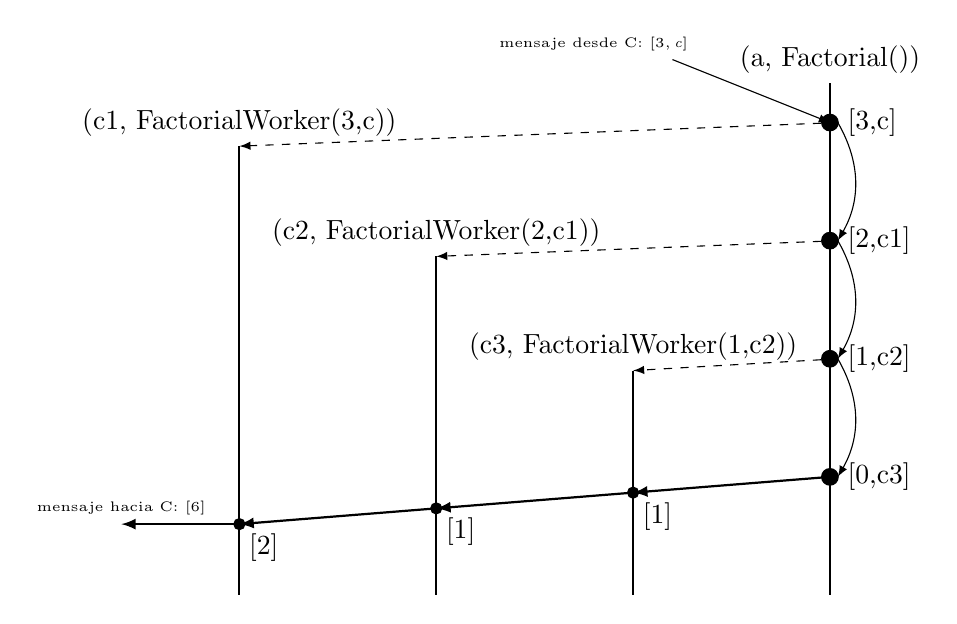
\begin{tikzpicture}

\draw[-latex] (6,7.3) to (8,6.5);

\draw[thick] (8,7) -- (8, 0.5);

\node[] at (5,7.5) {\tiny mensaje desde C: $[3,c]$};

\node[] (a1) at (8,7.3) {(a, Factorial())};

\node[align=center, right] (a1) at (8.1,6.5) {[3,c]};
\draw[fill] (8,6.5) circle (3pt);

\node[align=center, right] (a2) at (8.1,5) {[2,c1]};
\draw[fill] (8,5) circle (3pt);

\node[align=center, right] (a3) at (8.1,3.5) {[1,c2]};
\draw[fill] (8,3.5) circle (3pt);

\node[align=center, right] (a4) at (8.1,2) {[0,c3]};
\draw[fill] (8,2) circle (3pt);

\draw[-latex] (a1.west) to[bend left] (a2.west);
\draw[-latex] (a2.west) to[bend left] (a3.west);
\draw[-latex] (a3.west) to[bend left] (a4.west);

\node[] (d1) at (0.5,6.5) {(c1, FactorialWorker(3,c))};
\draw[thick] (d1.south) -- (0.5, 0.5);

\node[] (c1) at (3,5.1) {(c2, FactorialWorker(2,c1))};
\draw[thick] (c1.south) -- (3, 0.5);

\node[] (b1) at (5.5,3.65) {(c3, FactorialWorker(1,c2))};
\draw[thick] (b1.south) -- (5.5, 0.5);

\draw[fill] (5.5,1.8) circle (2pt);
\node[align=center, right] (b2) at (5.5,1.5) {[1]};

\draw[fill] (3,1.6) circle (2pt);
\node[align=center, right] (c2) at (3,1.3) {[1]};

\draw[fill] (0.5,1.4) circle (2pt);
\node[align=center, right] (d2) at (0.5,1.1) {[2]};

\draw[-latex, thick] (8,2)  -- (5.5,1.8);
\draw[-latex, thick] (5.5,1.8) -- (3,1.6);
\draw[-latex, thick] (3,1.6) -- (0.5,1.4);
\draw[-latex, thick] (0.5,1.4) -- (-1,1.4);

\draw[-latex, black, dashed] (a1.west) -- (d1.south);
\draw[-latex, black, dashed] (a2.west) -- (c1.south);
\draw[-latex, black, dashed] (a3.west) -- (b1.south);

\node[] at (-1,1.6) {\tiny mensaje hacia C: $[6]$};

\end{tikzpicture}

\caption{El diagrama ilustra el cálculo del factorial de 3. Todo el resultado es enviado al actor \textit{c}. Las líneas verticales indican el paso del tiempo, las de punto indican creación de actores y las otras flechas envío de mensaje. La lista superior indica la dirección del buzón y el tipo de actor con los parámetros con los que fueron inicializados.}

\label{fig:factorial}

\end{figure}

\subsection{Una pila usando actores}\label{sal:pila}

Otro ejemplo que podemos encontrar en \cite{Agha:1986:AMC:7929} es el de una pila, que está implementada con una lista enlazada. Se utiliza la dirección de un buzón como un puntero a un nodo de esta lista. 

Tiene dos operaciones básicas: apilar ($push$), que coloca un nodo en la pila, y su operación inversa, sacar ($pop$), que remueve el último elemento agregado en la pila.

\begin{lstlisting}[language=sal, style=simple]
def Node(content, link)
  case ['pop', customer]:
    send content to customer;
    become link;
  case ['push', newcontent]:
    let P = new Node(content, link)
      in become Node(newcontent, P)
end def

def Main() 
  let stack = new Node(10, Nil)
    in send [push, 20] to stack;
       send [push, 30] to stack;
  end
end
\end{lstlisting}

\begin{description}

\item [Línea 1] $Node$ recibe dos parámetros, $content$ que es un entero, el valor que tiene que guardar el nodo y  $link$ que es una dirección de buzón, es el siguiente actor en la pila.
\item [Línea 2] Si la operación es $'pop'$, guarda en $customer$ la dirección de buzón.
\item [Línea 3] Envía el contenido del nodo a la dirección de buzón $customer$
\item [Línea 4] La instrucción $become$, en este caso, hace que se reenvíen todos los mensajes a la dirección de buzón $link$. 
\item [Línea 5] Si la operación es $'push'$, guarda en $newcontent$ el valor del entero recibido.
\item [Línea 6] Crea un nuevo actor con los parámetros de inicialización $content$ y $link$.
\item [Línea 7] Asigna el siguiente comportamiento, como $Node$ con los parámetros $newcontent$ y la dirección de buzón del actor recién creado $P$. 
\item [Líneas 11-13] Crea una nueva pila con uno nodo con valor $10$, y envía dos operaciones $push$ con los valores $20$ y $30$.
\end{description}

El comportamiento $Node$ funciona como una lista enlazada, donde en vez de tener direcciones de memoria tenemos direcciones de buzón. El primer parámetro ($content$) es el contenido a guardar y el segundo ($link$) es el actor siguiente en la pila, o sea el puntero al siguiente elemento.

Cuando el primer valor de la lista es $pop$, se envía el valor que contiene el nodo al buzón $customer$ y se reenvían todos los mensajes a $link$. Todas las futuras operaciones $push$ y $pop$ las recibe este nodo, es decir que ahora es la ``cabeza'' de la pila. Esto guarda un parecido a mover un ``puntero''.

Cuando el primer valor de la lista es $push$, la pila crea un nuevo $node$ que será el nodo que quedará siguiente en la red. Se puede ver que esto ocurre en las líneas 7 y 8. Se copia en $P$ el nodo actual, y crea un nuevo nodo que es la nueva ``cabeza''.

Puede observarse en el ejemplo, que el primer nodo creado tiene como valor $Nil$, esto es simplemente una referencia nula. 

 % Actores
 
\documentclass[fleqn]{article}

\usepackage[utf8]{inputenc}
\usepackage{cite}

\usepackage{amsfonts}
\usepackage{amsmath}
\usepackage{amssymb}

\usepackage{hyperref}
\usepackage{syntax}
\usepackage{listings}
\usepackage{zed-csp}


\usepackage{tikz}
\usetikzlibrary{positioning}

\lstdefinelanguage{sal}{
  keywords = {send, become, let, new, in, to, if, then, else, case, def, end, case, of}
}

\lstdefinelanguage{csp}{
  keywords = {channel, datatype}
}

\lstdefinestyle{simple}{
  basewidth=0.5em
}



\title{CSP}
\author{José Luis Diaz}
\date{ }
 
\begin{document}
 
\maketitle
 
\tableofcontents
 
\section{Introducción}

\section{Conceptos básicos}

\subsection*{Comportamientos}

\subsection*{Creando Actores}

\subsection*{Creando comunicaciones}

\subsection*{Comandos}

\section{Lenguaje de Actor Mínimo}

Este lenguaje fue mostrado por primera vez en la tesis doctoral de Agha
\cite{Agha:1986:AMC:7929}, fue concebido como un lenguaje con fines pedagógicos.
Un programa en sal está compuesto por un conjunto \textit{Comportamientos}.
Como la mayoría de los lenguaje de programación, se agrega un
\textit{Comportamiento} llamado \textbf{main} como punto de entrada, está es una
adaptación de está tesina que no estaba originalmente.

\subsection{Comportamientos}

La sintaxis de los comportamientos es la siguiente:

\begin{grammar}
  <behavior> :== `def' <beh name> `(' <param-list> `)' `[`'<communication-list>`]' \\
            <command>* \\
  `end def'
\end{grammar}

La construcción \textit{param-list} es una lista de identificadores separados por coma,
se inicializan cuando el actor es creado. Por otra parte,
\textit{communication-list} contiene la comunicación a ser procesada por el
actor, esta puede ser una lista de identificadores.
Muchas veces dependiendo del tipo de comunicación que se esté enviando,
por ejemplo si el actor esta simulando ser una caja de ahorros, y recibe
un mensaje de \textbf{retirar} el mensaje debería contener la cantidad, pero en
caso de una consulta de saldo \textbf{balance} no debe especificar ningún parámetro
adicional, para esto se bifurca por el valor de uno de los campos llamado
\textbf{tag-field}, la sintaxis de esta puede  la siguiente:

\begin{grammar}
  <params> ::= <id> | <id> `,' <params>
  <var-list> ::= `case' <tag-field> `of' <variant>+ `end case'
  <variant> ::= <case label> `:' <params>
\end{grammar}

El siguiente ejemplo muestra un caso donde es útil utilizar la sintaxis basada
en \textbf{case}:

\begin{lstlisting}[language=sal, style=simple]
case pedido of 
  depositar: (cliente, monto) 
  retirar: (cliente, monto) 
  balance: (cliente) 
end case
\end{lstlisting}

No siempre es necesario utilizar esta sintaxis, \textit{communication-list} puede tener
la misma estructura que \textit{param-list}.

\subsection{Comandos}
La gramática de los comandos en SAL es la siguiente:

\begin{grammar}
  <command> ::= `send' $e_1, e_2, ..., e_n$ `to' <actor>  
  \alt `become' $B(e_1, e_2, ..., e_n)$
  \alt `let' $x_1$ = `new' $B_1(e_1, e_2, ..., e_{1n})$, \\
  ... $x_k$ = `new' $B_k(e_1, e_2, ..., e_{kn})$        \\
  `in' <command> 
  \alt `if`<bool-expr> `then' <command> `else' <command> `end if' 
  \alt <command> `;' <command>
\end{grammar}

\begin{description}
\item [send]  Este comando permite enviar mensajes a otros actores, toma como
  parámetro una lista separada por coma de las expresiones a enviar, y el actor
  destino, el envío de mensajes es asincrónico. Cada expresión es evaluada antes
  de ser enviada.
\item [become] Este comando especifica el siguiente comportamiento del actor
  que está procesando la comunicación recibida. Como en el caso anterior se evalúan
  las expresiones antes de ser enviadas, y estas aparecerán como la listas de
  parámetros del comportamiento. 
\item[new] Este comando sirve para crear nuevos actores. El alcance de los
  identificadores de los nuevos actores creados está sujeto a el cuerpo a del \textbf{let}.
\item[condicional] Luego de evaluar la expresión booleana, si es verdadera
  ejecuta lo que esta a continuación del \textbf{then}, en caso contrario lo que está a
  continuación del \textbf{else}. Funciona como cualquier condicional.
\item[secuenciación] Los comandos en sal ocurren al mismo tiempo, en este
  sentido podrían pensarse que los comandos de un comportamiento ocurren en paralelo.
  
\end{description}

\subsection{Expresiones}

Existen tres tipos primitivos, booleanos, enteros y dirección del buzón. Las operaciones
posibles entre los booleanos, \textbf{or}, \textbf{and}, \textbf{not}. Con
respecto a los enteros se pueden operar utilizando \textbf{+}, \textbf{-},
\textbf{*}, \textbf{/}. Un buzón es un identificador que es devuelto cuando se
crea un nuevo actor.

\subsection{Ejemplo: cálculo de factorial en SAL}

Está implementación del factorial está adaptada de \cite{Agha:1986:AMC:7929}, esta
depende de un actor \textit{main} que le envía el valor a calcular. El factorial
esta siempre disponible para procesar la siguiente comunicación, no bloquea con
el calculo recursivo del factorial sino que lo delega en otros actores.

La palabra reservada \textit{self} hace referencia a la dirección de buzón
correspondiente al actor que está procesando la comunicación, este es inicializado
cuando el actor es creado.

\begin{lstlisting}[language=sal, style=simple]
def Factorial()[val, customer]
  if val = 0 then
 send [1] to customer
  else
    let cont = new FactorialCont(val, customer)
       in send [val - 1, cont] to self
  end if
  become Factorial()
end def

def FactorialCont(n, customer)[arg] 
  send [n * arg] to customer
end def
\end{lstlisting}

El actor ante un entero distinto de cero ejecuta dos acciones, crea un actor con
un comportamiento que será multiplicar por \textbf{n} el valor recibido y
enviarlo al buzón de quien pidió el calculo del factorial de \textbf{n}.
También, se envía un mensaje a si mismo para evaluar el factorial de \textbf{n -
  1} y que le envíe el valor al actor que se acaba de crear. Este empeoramiento
se puede ver en la figura \ref{fig:factorial}.
En caso de que reciba \textbf{0} se le enviara \textbf{1} a quien pidió el
calculo del factorial.

\begin{figure}
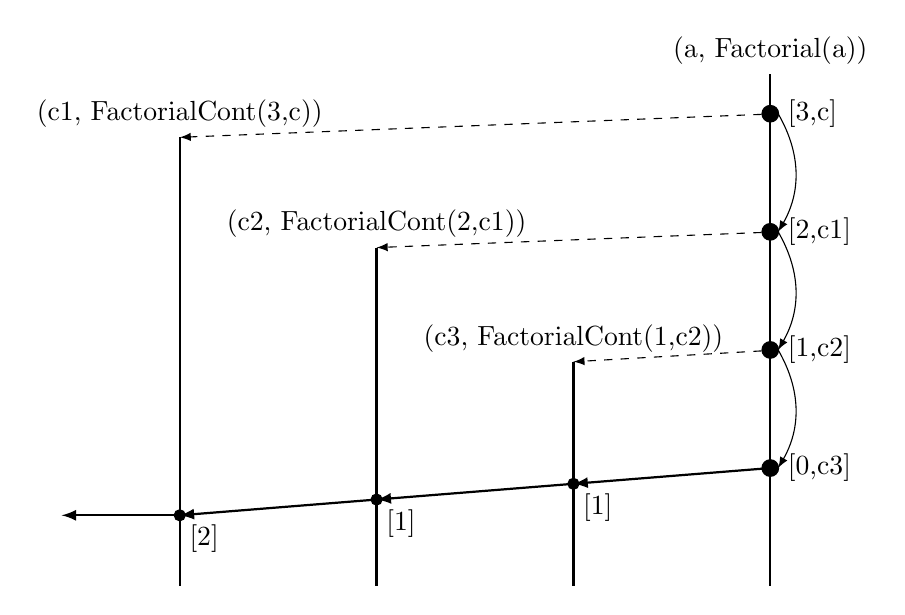
\begin{tikzpicture}
\draw[thick] (8,7) -- (8, 0.5);

\node[] (a1) at (8,7.3) {(a, Factorial(a))};

\node[align=center, right] (a1) at (8.1,6.5) {[3,c]};
\draw[fill] (8,6.5) circle (3pt);

\node[align=center, right] (a2) at (8.1,5) {[2,c1]};
\draw[fill] (8,5) circle (3pt);

\node[align=center, right] (a3) at (8.1,3.5) {[1,c2]};
\draw[fill] (8,3.5) circle (3pt);

\node[align=center, right] (a4) at (8.1,2) {[0,c3]};
\draw[fill] (8,2) circle (3pt);

\draw[-latex] (a1.west) to[bend left] (a2.west);
\draw[-latex] (a2.west) to[bend left] (a3.west);
\draw[-latex] (a3.west) to[bend left] (a4.west);

\node[] (d1) at (0.5,6.5) {(c1, FactorialCont(3,c))};
\draw[thick] (d1.south) -- (0.5, 0.5);

\node[] (c1) at (3,5.1) {(c2, FactorialCont(2,c1))};
\draw[thick] (c1.south) -- (3, 0.5);

\node[] (b1) at (5.5,3.65) {(c3, FactorialCont(1,c2))};
\draw[thick] (b1.south) -- (5.5, 0.5);


\draw[fill] (5.5,1.8) circle (2pt);
\node[align=center, right] (b2) at (5.5,1.5) {[1]};

\draw[fill] (3,1.6) circle (2pt);
\node[align=center, right] (c2) at (3,1.3) {[1]};

\draw[fill] (0.5,1.4) circle (2pt);
\node[align=center, right] (d2) at (0.5,1.1) {[2]};

\draw[-latex, thick] (8,2)  -- (5.5,1.8);
\draw[-latex, thick] (5.5,1.8) -- (3,1.6);
\draw[-latex, thick] (3,1.6) -- (0.5,1.4);
\draw[-latex, thick] (0.5,1.4) -- (-1,1.4);

\draw[-latex, black, dashed] (a1.west) -- (d1.south);
\draw[-latex, black, dashed] (a2.west) -- (c1.south);
\draw[-latex, black, dashed] (a3.west) -- (b1.south);

\end{tikzpicture}
\caption{El diagrama ilustra el cálculo del factorial de 3, todo el resultado es
enviado al actor \textit{c}. Las lineas en punto indican la creación de un actor.}
\label{fig:factorial}
\end{figure}

\section{CSP y actores}
Para empezar a describir como se modeló en CSP, primero es importante hacer
referencia a que se utilizó \textit{CSPm} \cite{fdr}, que combina los operadores de \textit{CSP}
originalmente propuesto por Hoare\cite{Hoare:1978:CSP:359576.359585}, y un lenguaje funcional.

En el proceso de traducción de \textit{SAL} a \textit{CSPm}, fue necesario construir un pequeño
\textit{runtime} para emular como los actores corren. Recordemos que la
naturaleza de \textit{CSP} es síncrona y los actores no lo son. Fue necesario
concretamente desacoplar la creación de nuevos actores, el envío y la recepción de mensajes. 

\subsection{Creación de nuevos actores}

Para desacoplar la creación de actores se utilizan varias abstracciones, en particular
\textbf{ActorID} y dos canales de \textit{CSP}.

Para definir \textbf{ActorID} utilizaremos tipos algebraicos parecidos a los de
haskell, soportados por \textit{CSPm}.

\[
datatype\ ActorID = Factorial.\{1\} | FactorialWorker.\{1,2,3\} | Main.\{1\}
\]

Este tipo introduce y nombra cada uno de los actores que van ser utilizados,
Aparte de incluir el nombre, también encapsula la cantidad de actores de un tipo
dado.
Para esto se utiliza la notacíon de conjunto que vemos entre llaves, en este
caso vamos a contar con un actor del tipo \textbf{Factorial}, tres del tipo
\textbf{FactorialWorker} y uno más del tipo \textbf{Main}.


\[
channel\ CreateAsk:ActorID.(Value, Value)\\
channel\ Create:ActorID.(Value, Value)
\]

Estos dos canales son los encargados de desacoplar la creación de un nuevo
actor. Aquí se introduce \textbf{Value}, un tipo de datos algebraico que
representa los valores que van ser pasado tanto en la creación de actores como en
el envío de mensajes. Los posibles valores a utilizar son enteros, \textbf{ActorID} o
\textbf{ATOMS}, este último se usa para denominar un tipo de cadena de
caracteres \footnote{//TODO: Agregar un apéndice mostrando todo el runtime?}. 

Para desacoplar el actor que tiene la intención de crear otro del creado, el primero
espera a sincronizar en un evento del tipo $CreateAsk$, como existe un proceso
auxiliar que está dispuesto encontrase con el, se libera y así puede continuar
el proceso que crea el nuevo actor. En realidad, la creación es algo ficticio ya
que tenemos una red de procesos \textit{CSP} esperando el evento $Create$ para
arrancar con el comportamiento definido.

\[
CreateAsk!FactorialWorker.1?m \then Create.FactorialWorker.1!m \then \Stop\\
CreateAsk!FactorialWorker.2?m \then Create.FactorialWorker.2!m \then \Stop\\
CreateAsk!FactorialWorker.3?m \then Create.FactorialWorker.3!m \then \Stop
\]


Este proceso simplemente espera a sincronizar con un evento de tipo
\textit{CreateAsk} y emite un evento de tipo \textit{Create}.
En la semántica de CSP cuando utilizamos \textbf{`?'} estamos esperando un
evento en un canal, si utilizamos \textbf{`!'} estamos enviando. Esto es una
notación ya que originalmente \textit{CSP} solo habla de dos procesos que se
encuentran en un punto dado.

En el ejemplo se puede ver que se envía el valor $FactorialWorker.1$ a quien esté
dispuesto a sincronizar, y se recepciona $m$ que es la tupla de valores antes
vista. Este punto es muy importante ya que se le esta enviando al proceso
que tiene la intención de crear un actor la dirección del buzón del nuevo actor
creado. Luego se espera a sincronizar con $Create.FactorialWorker.1$ a quien se
le envía el valor de $m$.

Esto no desacopla la creación que sino que, al mismo tiempo, La asignación de un
único nombre al actor. En este caso es el valor que se envía mediante
$CreateAsk$.

\subsection{Envío de mensajes}
Para desacoplar el envío de mensajes utilizamos una estructura intermedia que
actúa de \textit{buzón}, para comunicarase con esta estructura existen dos canales.

\[
channel\ CommSend:ActorID.(VALUE, VALUE)\\
channel\ CommRecv:ActorID.(VALUE, VALUE)
\]

Por cada actor en la red, existe un \textit{buzón} con el mismo \textbf{ActorId}
asociado a este. 
Un actor se bloquea esperando en $CommRecv$, cuando una nueva comunicación está
dispuesta a ser sincronizada, desde el \textit{buzón} hacia el actor esta es procesada.

Un \textit{buzón} puede guardar más de un mensaje en su interior. Esto
introduce un tipo de no determinismo, un actor puede sincronizar con cualquiera
de los mensajes disponibles en su \textit{buzón}.

El comportamiento del proceso buzón depende de su estado, si no tiene ningún
mensaje, si tiene algunos mensajes, o si está completo.
\begin{itemize}
\item Si no tiene ningún mensaje, solo sincroniza mensajes por el canal $CommSend$.
\item Si tiene algunos mensajes, por los canales $CommSend$ y $CommRecv$.
\item Si está completo, solo por el canal $CommRecv$.
\end{itemize}

Puede que los nombre de los canales suenen poco intuitivos, es importante notar que
provienen de la acciones vista desde los actores.

\begin{description}
\item [CommSend] Canal utilizado para comunicar desde cualquier actor hacia el buzón.
\item [CommRecv] Canal utilizado para comunicar del buzón hacia el actor asociado.
\end{description}

\subsection{Definición de comportamientos}
Para mostrar como funciona se utilizará un ejemplo simple, un actor que cuando
es creado recibe un parámetro del tipo \textbf{ActorId}, luego se queda esperando un
mensaje, cuando lo recibe, incrementa en uno el valor que este y lo envía al buzón de $a1$.

\[
  g = Create!G.1?(a1, None) \then g_{running}(G.1, a1) \\ 
g_{running}(self, ACTOR.client) = \\
\quad CommRecv.self!(INT.v, None) \then \\
\quad CommSend.client!(add(v, SI.1), None) \then \\ 
\quad g_{running}(self, ACTOR.client) \\
\]

Desarmando el ejemplo, una vez recibido el mensaje $Create!G.1?(a1, None)$,
podemos decir que el actor está \textit{Corriendo}, para marcar esta diferencia
se utiliza el proceso $g_{running}$.

Cuando un actor reacciona a una comunicación, tiene que definir el
comportamiento de reemplazo, en este caso puede ser el mismo comportamiento que
antes, o uno nuevo. Para esto útil separar, el actor antes de ser creado, del
actor que está corriendo. Sobre el final del ejemplo puede verse que se vuelve a
comportar como $g_{running}$.

Si no hubiera comportamiento de reemplazo simplemente la ultima linea sería
$\Stop$.

$CommRecv$ espera sincronizar con que el buzón propio al actor, cuando
recibe un mensaje, $CommSend.client$ envía una comunicación al buzón de $client$
el entero \footnote{Se utiliza una representación de enteros
  propios para evitar la explicación de estados que utilizar todos los enteros
  produce.} que recibió mas uno.


Para cerrar con esta idea, una implementación en \textit{SAL}.

\begin{lstlisting}[language=sal, style=simple]
def G(actor)[v]
    send [v + 1] to actor
end def
\end{lstlisting}

\subsection{Ejemplo: cálculo de factorial en CSPm}
Se utilizará el mismo ejemplo del factorial antes visto en sal \textbf{SAL},
está compuesto por dos comportamientos $Factorial$ y $FactorialWorker$.

\subsubsection*{Comportamiento de Factorial}

La primer parte del factorial es una suerte de preludio genérico que conecta un
actor que no está corriendo, o no fue creado con uno que fue creado. Esto es ya que
necesitamos arrancar toda la red de procesos en \textit{CSPm} en el momento de
comenzar la simulación.

\[
factorial = Create.Factorial.1?(None, None) \then factorial_{running}(Factorial.1) 
\]

En el caso de la formula anterior, espera a sincronizar con un mensaje de
creación. Esto no solamente simula la creación, sino que al mismo tiempo se
asigna el buzón con nombre $Factorial.1$ al actor que está corriendo. Dentro de
la definición del comportamiento hace referencia a $self$ como nombre de
su propio buzón.

Notar que en este caso solo necesita instanciar un solo actor de tipo $Factorial$.

\[
factorial_{running}(self) = CommRecv?self.(ACTOR.mailboxClient, INT.k) \then     \\
\textbf{if} (eq(k,SI.0)) \\
\quad  then \\
\quad \quad CommSend!mailboxClient.(INT.SI.1, None) \then factorialRunning(self) \\
\quad \textbf{else} \\
\quad \quad \textbf{let} \\
\quad \quad \quad newK = sub(k, SI.1) \\
\quad \quad \textbf{within} \\
\quad \quad \quad CreateAsk?FactorialWorker.pid!(INT.k, ACTOR.mailboxClient) \then \\
\quad \quad \quad CommSend!self.(ACTOR.FactorialWorker.pid, INT.newK)  \then \\
\quad \quad \quad factorial_{running}(self)
\]


El comportamiento del fragmento de código anterior es exactamente igual a él
código antes visto en \textit{SAL}. Cuando recibe un entero distinto de cero
ejecuta dos acciones, crea un actor \textbf{FactorialWorker} y se envía
un mensaje a si mismo para evaluar el factorial de \textbf{n - 1}.

En este caso el comportamiento de reemplazo para el buzón actual, es el mismo
que antes.

\subsubsection*{Comportamiento de FactorialWorker}

Antes de introducir el ejemplo, veamos como funciona la notación ${| |}$ de
\textit{CSPm}. Dado un tipo del $datatype T = A.{0..3}$, este es igual a
conjunto ${A.0, A.1, A.2, A.3}$, En vez de tener que enumerar todos los tipos de
$A$, podemos utilizar la notación ${|A|}$ que es equivalente.

En el caso del comportamiento de \textbf{FactorialWorker} vamos a necesitar
mas de un actor de este tipo, puede verse a continuación que se utiliza el operador de
interleaving de \textit{CSP} en conjunto con la notación anterior, para poner en
paralelo tantos procesos como elementos existan en el conjunto ${|FactorialWorker|}$.

\[
factorialWorker  = \Interleave_{x : \{|FactorialWorker|\}} Create!x?(k, mailboxClient) \\ 
\quad \then factorialWorker_{running}(x, k, mailboxClient)
\]

Utilizando esta notación el tipo de datos \textbf{ActorID}, tiene dos
responsabilidades: nombrar los actores y enumerarlos.
Recordemos que es necesario conocer la cantidad total de procesos que va
a tener un red de \textit{CSP} antes de comenzar la simulación.

\[
factorialWorker_{running}(self, INT.k, ACTOR.mailboxClient) = \\
CommRecv.self?(INT.n, None) \then \\
\quad \textbf{let} \\
\quad \quad val = mult(n, k) \\
\quad \textbf{within} \\
\quad \quad CommSend.mailboxClient!(INT.val, None) \then \\
\quad \Stop
\]


Este comportamiento es muy simple, en el momento de creación recibe dos
parámetros, un entero \textbf{k} y un dirección de un buzón, al momento de
recibir una comunicación, efectúa la multiplicación y se lo envía a
$mailboxClient$.
En este caso no cuenta con comportamiento de reemplazo, entonces termina con $\Stop$

\subsection{Ejemplo: Una pila en SAL}

Introducir el código en sal, y explicar como funciona.

\subsection{Ejemplo: Una pila en CSPm}

Introducir el código en CSPm equivalente y explicar las particularidades.

\subsection{Ejemplo: Un cliente-servidor de chat en SAL}

Introducir el código en sal, y explicar como funciona.

\subsection{Ejemplo: Un cliente-servidor de chat en CSPm}

Introducir el código en CSPm equivalente y explicar las particularidades.

\subsection{Traduciendo de SAL a CSPm}

Mostra la función que traduce de SAL a CSPm


TODO: Definir \textbf{translateExp}

La clase \textbf{Cmnd} con elementos de tipo S está dada por:

\begin{verbatim}
S :== S_1 ; S_2 | if b then S_1 else S_2 | send [e1, .., e_i] to a | become new
E(e_1, .. ,e_i) | let a_1 = new E_1(e_1,..,e_i) and ... a_j = new
E_1(e_1,..,e_i) { S } 
\end{verbatim}

definimos la funcion \textbf{translateCmd} de la siguiente forma:

\begin{verbatim}
translateCmd (S_1 S_2) = translateCmd(S_1) -> translateCmd(S_2)
\end{verbatim}


\begin{verbatim}
translateCmd(if b then S_1 else S_2) = 
   if (translateExp(b)) then
       translateCmd(S_1) else 
       translateCmd(S_2)
\end{verbatim}

\begin{verbatim}
translateCmd(send[e_1, ..., e_i] to a) = CommSend.a.
         (translateExp(e_1), ..., 
          translateExp(e_i)) 
\end{verbatim}

\begin{verbatim}
translateCmd(become new Beh(e_1, ..., e_n)) = runningBeh(self, e_1, ..., e_n)
\end{verbatim}

newEnv es el resultado de agregar a el entorno de las variables de mailbox $a_1
= E_1.pid_1$ .. $a_n = E_n.pid_n$
\begin{verbatim}
translateCmd(let a_1 = new E_1(e_1, ..., e_j) and 
         ... and a_n = new E_N(e_1, ..., e_j) { S } = 

CreateAsk?E_1.pid_1!(translateExp(e_1), ...,translateExp(e_j)) ->
CreateAsk?E_N.pid_n!(translateExp(e_1), ...,translateExp(e_j)) ->
translateCmd(S, newEnv)
\end{verbatim}


La clase \textbf{Beha} con elementos de tipo S está dada por:

\begin{verbatim}
def behName(a_1 .. a_i)[n_1 ... n_j]
  S
end def
\end{verbatim}

Tendria como equivalente en CSP:

\begin{verbatim}

behName = ||| actorId : {|BehName|} @ Create.actorId?(a_1, ..., a_i) ->
behNameRunning(actorId, a_1, .., a_n)

behNameRunning(self, a_1, .., a_n) = CommRecv.self(n_1 ... n_j) -> translateCmd(S)

\end{verbatim}

--- Agregar case? ---

\bibliography{references}{}
\bibliographystyle{plain}
\end{document}

 % SAL

% \chapter{Preliminares}

En en la primera sección de este capítulo se exploran algunas particularidades del paralelismo en \CSP, tales como, paralelismo sincrónico, alfabetizado, entrelazado y generalizado. En la segunda sección se muestran algunas construcciones en \CSPm que resultan útiles. 

La sección de \CSP no pretende ser una introducción al lenguaje; se asume que el lector tiene cierta familiaridad con él. Para una introducción se puede consultar \cite{Cristia:CSP}, para una referencia completa \cite{Roscoe:1997:TPC:550448}

\section{Algunas construcciones de CSP}

En esta sección se muestran algunos de los operadores de paralelismo de \CSP, seguido de algunos ejemplos de uso y su relación con el modelo de actores.  

\subsubsection*{Paralelismo sincrónico}

El operador más simple de \CSP es el que está dispuesto a sincronizar todos los eventos. Es decir, ambos procesos compuestos por este operador avanzan cuando encuentran un evento que ambos están dispuestos a sincronizar. Por ejemplo:

\begin{align*}
P_1 =& a \then P_1\\
P_2 =& a \then P_2 \\
SYSTEM =& P_1 \parallel P_2
\end{align*}
donde $P_1$ y $P_2$ sincronizan en el evento $a$. 

Cuando utilizamos procesos parametrizados muchas veces es útil enviar información. El siguiente ejemplo muestra esto:

\begin{align*}
P_1 =& canal!1 \then STOP \\
P_2 =& canal?x \then P(x) \\
SYSTEM =& P_1 \parallel P_2 \\
\end{align*}
donde $canal!1$ es quien envía el valor $1$ y $canal?x$ lo recibe. Para entender un poco más cómo funciona la notación que involucra $\langle ? \rangle$ y $\langle ! \rangle$, supongamos que $x$ puede tomar los valores $1$, $2$ y $3$. La expresión $canal?x$ equivale a un proceso que está dispuesto a sincronizar con todos estos potenciales valores:
\begin{align*}
P_2 & =  canal.1 \then STOP \\
      & \Extchoice canal.2 \then STOP \\
      & \Extchoice canal.3 \then STOP 
\end{align*}

Como $x$ es una variable libre y el evento que termina sincronizando es $canal.1$, ésta toma el valor $1$. En realidad el paso de información es ficticio; todo el tiempo se está sincronizando en eventos.

\subsubsection*{Paralelismo alfabetizado}

Mientras más procesos combinemos utilizando el operador $\parallel$, más procesos tienen que ponerse de acuerdo en los eventos a sincronizar si se pone en paralelo los procesos $P$ y $Q$ no necesariamente todas las comunicaciones de $P$ son para $Q$.

Si $X$ e $Y$ son dos conjunto de eventos, $P\ \textsubscript{X}\parallel\textsubscript{Y}\ Q$ es la composición paralela en donde $P$ tiene sólo permitido comunicar los eventos $X$ y donde $Q$ tiene sólo permitido comunicar los eventos $Y$, y únicamente tienen que ponerse de acuerdo en la intersección $X \cap Y$. Por ejemplo:

\[ 
 ( a \then b \then b \then STOP )\  \textsubscript{\{a, b\}} \parallel \textsubscript{\{b, c\}}\ ( b \then c \then b \then STOP ) 
\]

Se comporta como:

\[ 
 ( a \then b \then c \then b \then STOP )
\]

\subsubsection*{Entrelazado}
Los operadores $\parallel$ y $\textsubscript{X}\parallel\textsubscript{Y}$ tienen la propiedad que todos los procesos involucrados tienen que sincronizar algún evento. Utilizando el operador de entrelazado ($\Interleave$), cada proceso corre independiente de cualquier otro. Se nota $P \Interleave Q$.

\subsubsection*{Paralelismo generalizado}
Existe una forma general de escribir todos los operadores vistos utilizando el operador de paralelismo generalizado $P \Parallel\limits_{X} Q$, donde $P$ y $Q$ solo tienen que ponerse de acuerdo en los eventos pertenecientes a $X$ y los eventos que están por fuera de $X$ se procesan independientemente.

Podemos escribir el operador de entrelazado usando la siguiente equivalencia:

\[
 P \Interleave Q = P \Parallel\limits_{\{\}} Q
\]

Podemos escribir el operador de paralelismo alfabetizado como:

\[
 P\ \textsubscript{X}\parallel\textsubscript{Y}\ Q = P \Parallel\limits_{X \cap Y} Q
\]

Se puede definir el operador de paralelismo sincrónico de la siguiente forma, donde $\Sigma$ son todos los eventos posibles en un sistema dado.
\[
 P \parallel Q = P \Parallel\limits_{\Sigma} Q
\]

\subsubsection*{Cadena de caracteres}
\CSP no tiene soporte para cadena de caracteres, en esencia solo son procesos y eventos. Será util en el capítulo que se define el modelo poder utilizar dentro de las secuencias algún tipo de cadena de carácteres. Estas son inmutables y la única operación que se define sobre ellas es la comparación. Se representan utilizando una secuencia alfanumérica, encerradas entre comillas simples. Por ejemplo:
\begin{gather*}
'cadena1' \\
'cadena2' \\
\langle 'cadena1', 'cadena2' \rangle
\end{gather*}

\subsubsection*{Actores y CSP}\label{preliminares:actores}

Como vimos en el capítulo anterior, \CSP es sincrónico, mientras que el paso de mensajes o envío de comunicaciones en el sistema de actores no lo es. Si se quiere transmitir información entre dos procesos en \CSP lo escribimos (como vimos en el apartado de paralelismo sincrónico),de la siguiente forma:
\begin{align*}
P_1 =& canal!1 \then STOP \\
P_2 =& canal?x \then STOP \\
SYSTEM =& P_1 \Parallel P_2  
\end{align*}

Para poder desacoplar el envío de la recepción del mensaje, se puede utilizar una estructura intermedia de $BUFFER$, cuya especificación es:
\begin{align*}
BUFFER =& enviar?x \then recibir!x \then BUFFER \\
P_1 =& enviar!1 \then STOP \\
P_2 =& recibir?x \then STOP \\
SYSTEM =& ( P_1 \Interleave P_2 ) \Parallel BUFFER \\
\end{align*}

Como la comunicación es desde $P_1$ hacia $BUFFER$ y desde $BUFFER$ hacia $P_2$, no hay ninguna comunicación entre $P_1$ y $P_2$. Por esto se utiliza el operador de entrelazado.

En \CSP no existe el concepto de instancia, y se debe definir la red de procesos desde el comienzo. Es decir, no podemos crear nuevos procesos desde un proceso. Por lo tanto, simularemos la creación activando cada instancia mediante un evento especial. Para iniciar $n$ procesos de tipo $P$ se escriben los siguientes procesos en \CSP:
\begin{align*}
P =& \texttt{comportamiento-de-P} \then STOP \\
P_1 =& iniciar_1 \then P \\
P_2 =& iniciar_2 \then P \\
&\ldots \\
P_n =& iniciar_n \then P \\
SYSTEM =& P_1 \Interleave P_2 \Interleave \ldots \Interleave P_n
\end{align*}
donde $iniciar_i$ es el evento especial que da inicio a $P$. Se utiliza el operador de entrelazado para combinar los procesos $P_1, P_2, \ldots, P_n$, ya que no tiene que haber ninguna comunicación entre ellos. En el caso de existir algún evento compartido, este debería ser desestimado y no generar un encuentro. 
Con estos elementos podemos crear un proceso y enviar una comunicación de manera asincrónica. Se puede ver esto en el siguiente ejemplo:

\begin{align}\label{eq:smallactor}
\begin{split}
BUFFER_1 &= enviar.1?x \then recibir.1!x \then BUFFER_1\\
BUFFER_2 &= enviar.2?x \then recibir.2!x \then BUFFER_2\\
SUMA &= inicia_{suma} \then recibir.1?x \then enviar.2!(x + 1) \then STOP \\
CLIENTE &= inicia_{suma}\then enviar.1!2 \then recibir.2?x \then STOP \\
BUFFER &= BUFFER_1 \Interleave BUFFER_2 \\
SYSTEM &= (SUMA \Parallel\limits_{\{inicia_{suma}\}} CLIENTE) \Parallel\limits_{Y}\ BUFFER
\end{split}
\end{align}

Es decir que $CLIENTE$ inicia el proceso $SUMA$, y le envía un $2$. Este envío es asíncrono por $BUFFER_1$. Cuando $SUMA$ recibe este $2$, crea una nuevo mensaje y se lo envía a $CLIENTE$ de manera asincrónica, con el valor que recibió incrementado en uno. En la composición de $SYSTEM$ se puede ver que el único evento que se sincroniza entre $SUMA$ y $CLIENTE$ es $inicia_{suma}$. En el otro operador paralelo, los valores de $Y$ vienen dados por los eventos en los que la composición de $SUMA$ y $CLIENT$ sincronizan con $BUFFER$. Para esto deberíamos saber qué valores puede tomar $x$. Asumiendo que toma los valores $1$, $2$ y $3$. Los eventos a sincronizar serían el conjunto generado por $\{m: [1,2] ,n: [1,2,3] | recibir.m.n \} \cup \{m: [1,2] ,n: [1,2,3] | enviar.m.n \} $, es decir todos los eventos inherentes a $BUFFER$.

Este último ejemplo muestra dos de los aspectos que se desarrollarán en el capítulo siguiente: cómo desacoplar el envío de mensajes y cómo simular la creación de un proceso. También puede verse el uso de los distintos operadores paralelo.
 
\section{El lenguaje CSPm}

\CSPm es un lenguaje funcional, que tiene una integración para definir procesos de \CSP. También permite realizar aserciones sobre los procesos de \CSP resultantes. Este lenguaje es el que utiliza la plataforma \FDR. En esta sección se describirán algunas de las construcciones de \CSP en \CSPm y algunas construcciones propias de \CSPm.

\subsubsection{Tipos algebraicos}

Permite declarar tipos estructurados, son similares a las declaraciones de tipo \textit{data} de Haskell. La más simple de las declaraciones es utilizando constantes.

\begin{verbatim}
datatype ColorSimple = Rojo | Verde | Azul
\end{verbatim}

Esto declara \verb=Rojo=, \verb=Verde= y \verb=Azul=, como símbolos del tipo \verb=ColorSimple=, y vincula \verb=ColorSimple= al conjunto \verb={Rojo, Verde, Azul}=. Estos tipos de datos puede tener parámetros. Por ejemplo, se pude agregar un constructor de datos \verb=RGB=, a saber:

\begin{verbatim}
datatype ColorComplejo = Nombre.ColorSimple | RGB.{0..255}.{0..255}.{0..255}
\end{verbatim}

Esto declara \verb=Nombre=, como un constructor de datos, de tipo \verb=ColorSimple= $\Rightarrow$ \verb$ColorComplejo$ y a \verb$RGB$ como un constructor de datos de tipo \verb$Int$ $\Rightarrow$ \verb$Int$ $\Rightarrow$ \verb$Int$ $\Rightarrow$ \verb$ColorComplejo$ y \verb$ColorComplejo$ es el conjunto:
\begin{multline*}
\{ Nombre.c | c \leftarrow  ColorSimple \} \cup \{ RGB.r.g.b |  r \leftarrow \{ 0 \dots 255 \},  g \leftarrow \{ 0 \dots 255 \}, \\  b \leftarrow \{ 0 \dots 255 \} \}  
\end{multline*}

Si se declara un tipo de datos T, entonces a T se adjunta el conjunto de todos los valores de tipo de datos posibles que se pueden construir. 

\subsubsection{Canales}

Los canales de \CSPm son utilizados para crear eventos, y se declaran de una manera similar a los tipos de datos. Por ejemplo:

\begin{verbatim}
channel estaListo
channel x, y : {0..1}.Bool
\end{verbatim}

Declara tres canales, uno que no toma parámetros (listo es de tipo Event), y dos que tienen dos componentes. Cualquier valor del conjunto \verb={0,1}= y un booleano. El conjunto de los eventos definidos es el siguiente: 
\begin{verbatim}
	
\end{verbatim}
\verb={ estaListo, x.0.false, x.1.false, x.0.true, x.1.true, y.0.false, y.1.false, y.0.true, y.1.true }=. Estos eventos pueden ser parte de la declaración de procesos como por ejemplo \verb#{P = x?a?b -> STOP}#.

\subsubsection{Búsqueda de patrones}

Es posible en \CSP que los valores puedan ser buscados por coincidencia de patrones. Por ejemplo, la siguiente función toma un entero, se puede usar en la búsqueda de patrones para especificar un comportamiento diferente dependiendo de este argumento:

\begin{verbatim}
f(0) = True
f(1) = False
f(_) = error("Error")
\end{verbatim}

Funciona de manera similar a Haskell, también se pueden utilizar otras construcciones como secuencias o algún tipo algebraico.

\subsubsection{Operadores replicados}
\FDR tiene una versión replicada o indexada de alguno de sus operadores. Estos proveen una forma simple de construir un proceso que consiste en una serie de procesos compuestos utilizando el mismo operador. Por ejemplo se define P de la siguiente manera, \verb=P :: (Int) -> Proc= luego, \verb=||| x: { 0..2 } @ P(x)= evalúa P para cada valor de x en el conjunto dado y los compone utilizando el operador de entrelazado. Por lo tanto, lo anterior es equivalente a \verb=P (0) ||| P (1) ||| P (2)=.


La forma general de un operador replicado es:

\begin{verbatim}
op <declaraciones> @ P
\end{verbatim}

donde op es un operador que puede ser el de entrelazado, selección interna, etc. P es la definición de un proceso, puede hacer uso de las variables definidas por las declaraciones. Cada uno de los operadores evalúa P para cada valor que toman las declaraciones antes de componerlas juntas usando op.

En \CSPm las declaraciones puede ser construcciones por comprensión, cómo las que generan nuevos conjuntos basados en conjuntos existentes. Por ejemplo, el conjunto por comprensión: \verb={x + 1 | x <- xs}= incrementa cada elemento del conjunto xs en 1. 

Otra forma de construcción por compresión es utilizar la siguiente expresión: \verb={| CANAL |}=, que genera el conjunto de todos los elementos del canal. Por ejemplo, dada la siguiente definición de canal \verb=channel X : {0..1}.Bool=, el conjunto generado por \verb={| X |}=es: \verb={X.0.false, X.0.true, X.1.false, X.1.true}=.



\subsubsection{Otras construcciones}
En esta sección se muestran algunas de las conversiones útiles para entender un programa en \CSPm.

Tabla de conversión para secuencias:

\begin{center}
\begin{tabular}{ l l }
  $\seq$ a & \verb|Seq(a)| \\
  $\nil$ & \verb|< >| \\
  $\langle 1, 2, 3 \rangle$ & \verb|<1,2,3>| \\
  $\Nil s$ & \verb=Null(s)=
  \\
  $s \cat t$ & \verb=s^t=
  \\
  $\# s$ & \verb|#s|
  \\
  $head~s$ & \verb|head(s)|
  \\
  $tail~s$ & \verb|tail(s)|
  \\
  $\dcat s$ & \verb|concat(s)|
  \\
  $x \elem s$ & \verb=elem(x,s)=
  \\
  $\ran s$ &  \verb|set(s)|
  
\end{tabular}
\end{center}

Tabla de conversión para la definición de procesos:

\begin{center}
\begin{tabular}{ l l }
  Stop & \verb=STOP= \\
  Skip & \verb=SKIP= \\
  $c \then p$ & \verb=c -> p= \\
  $c ? x  \then p$  & \verb=c?x -> p= \\
  $c ! v \then p$ & \verb=c!v -> p= \\
  $p \extchoice q$ & \verb=p [] q= \\
  $p \intchoice q$ & \verb=p |~| q= \\
  $p \interleave q $ & \verb=p ||| q= \\
  $p \parallel q $ & \verb=p || q= \\
  $p\ \textsubscript{X} \parallel \textsubscript{Y}\ q$ & \verb=p |[|X|]| q= \\
  $p \Parallel\limits_{X} q$ & \verb=p |[x||y]| q= \\
  \end{tabular}
\end{center}

 % Preliminares de CSP?

\chapter{Un modelo en CSP}
En este capítulo se modela un sistema de actores utilizando \CSP. Este incluye las funciones definidas por \SAL, que se comentaron previamente. Tales como crear nuevos actores, enviar mensajes, y definir un comportamiento de reemplazo. 

Se comienza por una descripción detallada de cada componete, algunos ejemplos de traducción de \SAL a \CSP. Se presenta una función que traduce de \SAL a \CSP. Para terminar con algunas particularidades sobre el modelo propuesto al utilizar la herramienta \FDR.

\section{Describiendo el sistema de actores} 
Dentro de las acciones que un actor efectúa está la de crear otro actor. En \CSP los actores corresponden a procesos, como todos los procesos tienen que estar definidos desde el comienzo, en \CSP no existe la posibilidad de crear dinámicamente un nuevo proceso.

Se simula la creación definiendo cada proceso con la espera de un mensaje que de inicio. Esto podría verse como la palabra reservada $new$ en varios lenguajes de programación orientados a objetos. 

\subsection{Buzón}\label{modelo:buzon}

Recodemos que la naturaleza de \CSP es sincrónica y los actores no lo son. Para esto se necesita desacoplar el envío de mensajes de la recepción. Se utiliza una estructura intermedia que actúa de \textit{buzón}, y dos canales que sirven para comunicarse con ella.

La ecuación de \textit{buzón} es la siguiente:

\begin{process}
\begin{block}
Mailbox(i, \nil) = {} \\ \quad
CommSend?i.x \then Mailbox(i, \lseq x \rseq) 
\end{block} \\

\begin{block}
Mailbox(i, \lseq x \rseq \cat xs ) = {} \\ \quad 
  \begin{block}
    CommRecv!i.x \then Mailbox(i, xs) \\
    \Extchoice \\
    CommSend?i.y \then Mailbox(i, \lseq x \rseq \cat xs \cat \lseq y \rseq ) 
  \end{block}
\end{block} \\

\end{process}

Donde $Mailbox(i, \nil)$ es cuando \textit{buzón} está vacío. $Mailbox(i, \lseq x \rseq \cat xs )$ es cuando tiene al menos un mensaje. Los canales para comunicarse con el buzón se definen de la siguiente forma:

\begin{align*}
channel\ CommSend:mailboxId.params \\
channel\ CommRecv:mailboxId.params
\end{align*}

Donde:
\begin{description}
 \item $channel\ CommSend:mailboxId.params$ define el canal $CommSend$. El primer parámetro es cualquier $mailboxId$ y representa el mailbox destino. El segundo parámetro, es una lista. Representa las comunicaciones enviadas. 
 \item $channel\ CommRecv:mailboxId.params$ define el canal $CommRecv$. Los parámetros son idénticos a los anteriores.
\end{description}

Un \textit{buzón} puede guardar más de una comunicación en su interior. Las comunicaciones se agregan al final, y se consumen sobre el principio. En este sentido, es una cola d tipo FIFO, del acrónimo inglés de First In, First Out (``primero en entrar, primero en salir'').

El comportamiento del proceso buzón depende de su estado, si no tiene ningún mensaje, o si tiene al menos algún mensaje. 

\begin{itemize}
\item Si no tiene ningún mensaje, solo sincroniza mensajes por el canal $CommSend$.
\item Si tiene algunos mensajes, por los canales $CommSend$ y $CommRecv$.
\end{itemize}

Puede que los nombre de los canales suenen poco intuitivos, es importante notar que provienen de la acciones vista desde los actores.

\begin{description}
\item $CommSend$ canal utilizado para comunicar desde cualquier actor hacia el buzón.
\item $CommRecv$ canal utilizado para comunicar del buzón hacia el actor asociado.
\end{description}

Por cada actor en la red, existe un \textit{buzón} con el mismo $mailboxId$ asociado. Para esto utilizamos la siguiente ecuación:

\[
Mailboxes = \Interleave_{ actor : MailboxIDS } Mailbox(actor, \nil) 
\]

Donde $Mailboxes$ representa todos los buzones puestos en paralelo utilizando el operador \textit{Interleave}. Como no existe comunicación entre buzones, siempre la comunicación es desde un actor hacia un buzón es que se elige el operador de \textit{Interleave}. $MailboxIDS$ es un conjunto de enteros, este representa un identificador único para los buzones. Tendrá que tener tantos elementos, como actores sean necesarios. Esto se verá en las siguientes secciones. 


\subsection{Identificadores de actores}\label{model:id}

Ya que no existe en \CSP el concepto de instancia es necesario contar con todos los procesos que van a ser parte de la red definidos desde el principio. El valor $N_i$ corresponde a la cantidad de actores de este tipo que van a ser necesarios. 


\subsection{Crear nuevos actores}\label{modelo:crear}

Para identificar que actor se está queriendo crear, se utiliza un conjunto con los nombres de los actores que van a ser creados. 

\begin{align*}
  ActorID &= { ACTOR_1, ACTOR_2, \ldots, ACTOR_K, MAIN }
\end{align*}

En \CSP no existe el concepto de instancia, y debemos tener definida la red de procesos desde el comienzo. Para resolver este problema, se presentan a continuación un dos abstracciones.

La primera abstracción es un preámbulo a un comportamiento, le asigna a este los parámetros \textit{acquaiantence-list} y al mismo tiempo le otorga al actor su identificador único de \textit{buzón}. Utilizamos para esto un conjunto de procesos puestos en paralelo, y un canal para comunicarse con ella.

El canal para comunicarse con los procesos que están esperando ser iniciados, se define de la siguiente forma:

\[
channel\ Create:actorid.mailboxid.params
\]

Donde $channel\ Create:actorid.mailboxid.params$ define el canal $Create$. El primer parámetro es cualquier $ActorID$, representa el actor a ser creado. El segundo parámetro es el identificador de buzón. El tercer parámetro, es una lista. Representa los identificadores \textit{acquaiantence-list}. 

\begin{align*}
ks = \Interleave_{i: \{1 .. N\_KS\}} & Create.k?self?<p1, p2> \then \\
& K(self, p1, p2) 
\end{align*}

Donde:

\begin{itemize}
 \item $ks$ es el conjunto de todos los procesos puestos en paralelo.
 \item $N\_KS$ define la cantidad de actores de tipo $K$ que se van a estar disponibles.
 \item $Create.k?self?<p1, p2>$, sincroniza en el canal $Create.k$ recibe el identificador de buzón $self$ como parámetro y la lista  $<p1, p2>$. En este caso estamos suponiendo que $K$ tiene solo dos parámetros de tipo \textit{acquaiantence-list}.
 \item $K(self, p1, p2)$ llama al proceso parametrizado definido como $K$ con los parámetros $self$, $p1$ y $p2$. $K$ representa el comportamiento del actor
\end{itemize}

En realidad, la creación es algo ficticio, ya que tenemos una red de procesos \CSP esperando al evento $Create.k$ para arrancar con el comportamiento definido. 

%El conjunto definido por $ACTOR_k$ es equivalente a los elementos definidos en $ActorID$. Por esto es que decimos que no sólo define el nombre, sino que al mismo tiempo está estableciendo cuantos actores del tipo $ACTOR_k$ se va a tener.

El proceso que representa a todos los actores que van a ser iniciados en paralelo, utiliza el operador de \textit{Interleave}. Una vez sincronizado en el mensaje $Create$, se ejecuta el comportamiento que obtiene el identificador del buzón y los parámetros recibidos. 

La segunda abstracción es un proceso que vuelve asincrónica el mensaje de creación, de la creación como tal. Para esto se utiliza una estructura intermedia $create$ y un canal para comunicarse con ella. $create$ se define de la siguiente forma: 

\[
\begin{array}{l}
Create(mailboxId) = CreateAsk?actorId!mailboxId?m \then Create.actorId?mailboxId!m \then STOP \\
Creates = \Interleave_{mailboxId : MailboxIDS} create(mailboxId)
\end{array}
\]

Donde:

\begin{description}
 \item $Create(mailboxId)$ es un proceso parametrizado.
 \item $CreateAsk?actorId!mailboxId?m$ sincroniza en el canal $CreateAsk$. Recibe $actorId$, el identificador de actor a crear. Envía el identificador de buzón $MailboxID$ y recibe la lista de valores $m$
 \item $\Interleave_{mailboxId : MailboxIDS}$ pone en paralelo tantos procesos en paralelos, como elementos definidos en $MailboxIDS$.  
\end{description}

El canal para comunicarse con esta estructura se define como:

\[
channel\ CreateAsk:actorid.mailboxId.params
\]

Donde: $channel\ CreateAsk:actorid.mailboxId.params$ define el canal $CreateAsk$, el primer parámetro es cualquier $ActorID$, representa el tipo de actor a ser creado. El segundo parámetro representa la dirección de buzón y el tercer parámetro, es una lista. Representa los identificadores \textit{acquaiantence-list}. 

Como puede observarse, tenemos tantos procesos en paralelo como elementos $MailboxIDS$ existan. Tal vez esta abstracción podría haber sido omitida, pero juega un papel fundamental en la construcción total del sistema, esto tiene que ver con en \CSP se puede elegir los eventos \cite[chap.~2,p.~55]{Roscoe:1997:TPC:550448} que se van a sincronizar, cuando como se compone todo el sistema, esta idea quedará más clara.

\subsection{Definición de comportamientos}
La idea de comportamiento fue introducida en la sección \ref{actores:beha}, podemos pensar a un comportamiento como una función que procesa una comunicación y tiene como salida, nuevas comunicaciones, nuevos actores y el comportamiento de reemplazo para el actor que esta procesando la comunicación.

\begin{align*}
&CommSend.d!<p_1, p_2, \ldots, p_n> & (Enviar\ Comunicaciones) \\ 
&CreateAsk.actor_m.buzon?<p_1, p_2, \ldots, p_m> & (Crear\ nuevos\ actores)\\
&K(self, p_1, p_2, \ldots, p_m)  & (Comportamiento\ de\ reemplazo)
\end{align*}

\begin{description}
\item [Enviar comunicaciones] En este caso le enviaremos al actor con la dirección buzón $d$ la listas de valores $<p_1, p_2, \ldots p_n>$. 
\item [Crear nuevos actores] Se crearía un actor con comportamiento $actor_m$ y obtendríamos mediante $buzon$ el identificador de buzón, y le asignarían los parámetros $<p_1, p_2, \ldots p_m>$ como \textit{acquaiantence-list}.
\item [Comportamiento de reemplazo] En este caso el comportamiento sería $K$. De no contar con uno sería simplemente $STOP$.
\end{description}

\section{Ejemplos}

En esta sección se muestran cuatro ejemplos. Los dos primeros son los vistos en la sección \ref{sal:factorial} y \ref{sal:pila} modelados en \CSP en vez de \SAL. Los siguientes dos son nuevos, uno es la estructura de datos \textbf{cola} y el otro un ejercicio tomado del libro \textit{Programming Erlang}\cite{Cesarini:2009:EP:1717841}.

\subsection{Ejemplo: cálculo de factorial en CSP}
En esta sección se describe el funcionamiento del factorial. Es una implementación en \CSP del ejemplo antes visto en \SAL. Está compuesto por dos comportamientos $Factorial$ y $FactorialWorker$.

Continuando con la mecánica del capítulo anterior, primero se presenta el código en \CSP, luego se comentan las líneas de interés, para terminar con un pequeño detalle del funcionamiento.

El primero de los comportamientos, es el de $Factorial$ que viene dado por la siguiente forma:
\begin{process}
Factorial(self) = {} \\ \quad
  \begin{block}
  CommRecv?self.\langle mailboxClient, k \rangle \then {} \\ \quad
    \begin{block}
    \If (k == 0) \Then {} \\ \quad
      \begin{block} 
      CommSend!mailboxClient.\langle 1 \rangle \then \\
      Factorial(self) 
      \end{block} \\
    \Else {} \\ \quad
      \begin{block}
      CreateAsk.factorialWorker?pid!\langle k, mailboxClient \rangle \then \\
      CommSend!self.\langle pid, k - 1 \rangle \then \\
      Factorial(self)
      \end{block}
    \end{block}
  \end{block}
\end{process}


\begin{description}
 \item $CommRecv?self.<mailboxClient, k>$ espera recibir una comunicación con los parámetros de tipo, el primero buzón y el segundo un entero.
 \item $\If (k == 0)$ Compara $k$ con el valor cero.
 \item $CommSend!mailboxClient.\langle 1 \rangle$ envía una comunicación al buzón $mailboxClient$ la lista con el valor $1$.
 \item $CreateAsk.factorialWorker?pid!\langle k, mailboxClient \rangle$ crea un nuevo actor de tipo $FactorialWorker$, guarda en $pid$ la dirección del buzón. Inicializa los valores \textit{acquaiantence-list} con el entero $k$ y el buzón $mailboxClient$.
 \item $CommSend!self.<pid, k - 1 >$ Se auto envía un mensaje, con el valor de buzón del actor creado en la linea anterior, y el entero $k$ decrementado en uno.
 \item $Factorial(self)$ define como siguiente comportamiento, $Factorial$ para el buzón $self$.
\end{description}

Cuando recibe un entero distinto de cero ejecuta dos acciones, crea un actor \textbf{FactorialWorker} y se envía un mensaje a si mismo para evaluar el factorial de \textbf{n - 1}. En este caso el comportamiento de reemplazo para el buzón actual no cambia. Para una descripción mas detallada revisar la sección \ref{sal:factorial}

El segundo de los comportamientos, es el de $FactorialWorker$ que viene dado de la siguiente forma:

\begin{process}
FactorialWorker(self, k, mailboxClient) = {} \\ \quad
  \begin{block}
  CommRecv.self?\langle n \rangle \then {} \\ \quad
    \begin{block}
    CommSend.mailboxClient!\langle n * k \rangle \then \\
    STOP
    \end{block}
  \end{block}
\end{process}

\begin{description}
 \item $CommRecv.self?\langle n \rangle$ Espera una comunicación que contenga un entero, y lo guarda en $n$.
 \item $CommSend.mailboxClient!\langle n * k \rangle$ envía el resultado de la multiplicación a la dirección de buzón $mailboxClient$
\end{description}

Este comportamiento es muy simple, en el momento de creación recibe dos parámetros, un entero $k$ y un dirección de un buzón. Al momento de recibir una comunicación, efectúa la multiplicación del valor recibido por $k$ y se lo envía a $mailboxClient$.

En este caso no cuenta con comportamiento de reemplazo, entonces termina con $STOP$.

Tanto para $Factorial$ y para $FactorialWorker$ faltan definir los procesos que van a dar inicio a los actores. Los cuales se encuentran definidas en la sección \ref{modelo:crear}. 

\subsection{Ejemplo: Una pila}
En este ejemplo se construye una estructura de datos de tipo \textbf{pila}, la cual está compuesta de un solo comportamiento $node$ que es el que se encarga de recibir las operaciones $'push'$ y $'pop'$. En este caso se agrega al modelo $fwd$ que como veremos, está encargado de modelar el comportamiento $\textbf{become}\ buzon$.

El comportamiento de $fwd$ está definido de la siguiente forma:

\[
  fwd(a, b) = CommRecv.a?msg \then CommSend.b!msg \then fwd(a, b)
\]

El proceso anterior, reenvía todas las comunicaciones desde el buzón de $a$, al buzón de $b$.

El comportamiento de $node$ está definido de la siguiente forma:

\begin{process}
Node(self, content, link) = {} \\ \quad
\begin{block}
CommRecv.self?\langle 'push', newContent \rangle \then \\
CreateAsk.node?newNode!\langle content, link \rangle \then \\
Node(self, newContent, newNode)
\end{block} \\
\Extchoice \\ \quad
\begin{block}
CommRecv.self?\langle 'pop', client \rangle \then  \\
CommSend.client!\langle content \rangle \then  \\
fwd(self, link)
\end{block}

\end{process}

Donde:

\begin{description}
 \item $CommRecv.self?\langle 'push', newContent \rangle$ espera recibir un mensaje, donde el primer elemento de la lista es la constante $'push'$. Guarda en $newContent$ el valor del segundo elemento de la lista.
 \item $CreateAsk.node?newNode!\langle content, link \rangle$ crea un actor de un tipo $Node$ y guarda en $newNode$ el valor de la dirección del buzón. Inicializa los valores \textit{acquaiantence-list} con valor $content$ y el buzón $link$.
 \item $Node(self, newContent, newNode)$ define como comportamiento para el buzón $self$, el mismo comportamiento con los parámetros, $newContent$ y el buzón creado en la linea anterior.
 \item $CommRecv.self?\langle 'pop', client \rangle$ espera recibir un mensaje, donde el primer elemento de la lista sea la constante $'pop'$, guarda en $client$ el valor del segundo elemento de la lista.
 \item $CommSend.client!\langle content \rangle$ envía una comunicación al buzón $client$ la lista con el valor $content$.
 \item $fwd(self, link)$ se comporta como el proceso $fwd$.
\end{description}

Cuando la operación es de tipo $'pop'$, se envía el valor que contiene el nodo al buzón $client$ y se reenvían todos los mensajes a $link$, todas las futuras operaciones $'push'$ y $'pop'$ las recibe este nodo.

Cuando la operación es de tipo $'push'$, la pila crea un nuevo actor $node$. Se copia en $Node.newNode$ el nodo actual, y se reemplaza el contenido del nodo actual con el contenido recibido. Esto puede verse como el reemplazo de la cabeza de la pila.

\subsection{Ejemplo: una cola}\label{ejemplo:cola}

En este ejemplo se explora cómo construir una estructura de datos de tipo \textit{cola}, la cual se modela como si fuera una máquina de estados, dónde cada comportamiento corresponde a un estado y las comunicaciones son quienes disparan las transiciones de estos. Primero se muestra el ejemplo escrito utilizando \SAL, y luego su equivalente en \CSP.

Existen dos operaciones posibles para efectuarse en una \textit{cola} $QUEUE$ o encolar, y $DEQUEUE$ o desencolar. La primera operación agrega un nodo al final, y la segunda lo remueve del principio. 

Tanto el ejemplo en \SAL como el de \CSP tienen cuatro comportamientos:

\begin{description}
 \item [node] Guarda el contenido y una referencia al siguiente nodo en la \textit{cola}, son los eslabones de construcción de una suerte de lista enlazada.
 \item [queue] Quien se encarga de gestionar los nodos. Tiene referencia a dos nodos, el primero y el último. Para poder remover el primero, y agregar sobre el final.
 \item [emptyQueue] Este es el comportamiento es cuando la \textit{cola} no tiene ningún nodo en ella.
 \item [waitDelete] Un estado transicional, es utilizado cuando se elimina un nodo de la \textit{cola}.
\end{description}

En el resto de la sección se detallaran cada uno de los cuatro comportamientos antes enumerados, para terminar con una descripción de como estos funcionan en conjunto.

\subsubsection*{Comportamiento de node}
Este comportamiento es el que está encargado de guardar el contenido que se quisiera guardar en la \textit{cola}. Consta de dos operaciones $'delete'$ e $'point\_to'$. La primer operación envía todo su contenido a una dirección de buzón y termina su ejecución. El segundo, cambia el valor de $link$.

Código en \SAL:

\begin{lstlisting}[language=sal, style=simple]
def Node(content, link) match
  ['delete', mailbox]:
    send [content, link] to mailbox
  ['point_to', newLink]:
    become Node(content, newLink);
end def
\end{lstlisting}

Donde:

\begin{description}
 \item [Líneas 2-3] Si la operación es $'delete'$, envía su contenido a $mailbox$. Como no hay comportamiento de reemplazo, este nodo termina su ejecución en este momento.
 \item [Líneas 4-5] Si la operación es $'point\_to'$, el comportamiento de reemplazo tiene un nuevo nodo al que apunta. Esta operación básicamente cambia, el nodo que está próximo en la \textit{cola}.
\end{description}

Código en \CSP:

\begin{process}
Node(self, content, link) = \\ \quad
  \begin{block}
  CommRecv.self?\langle 'delete', mailbox \rangle \then \\
  CommSend.mailbox!(content, link) \then \\
  STOP
  \end{block} \\

  \Extchoice \\ \quad
  
  \begin{block}
  CommRecv.self?\langle 'point\_to', newLink\rangle \then \\
  Node(self, content, newLink)
  \end{block}
\end{process}

Donde: 

\begin{description}
 \item $CommRecv.self?\langle 'delete', mailbox \rangle$ espera recibir un mensaje, donde el primer elemento de la lista sea la constante $'delete'$. Guarda en $mailbox$ el valor del segundo elemento de la lista, que es una dirección de buzón.
 \item $CommSend.mailbox!\langle content, link \rangle$ Envía una comunicación al buzón $mailbox$, con la lista $content$ y $link$.
 \item $STOP$ Al no haber comportamiento de reemplazo, el actor termina su ejecución.
 \item $CommRecv.self?\langle 'point\_to', newLink \rangle$ Espera recibir un mensaje, donde el primer elemento de la lista sea la constante $'point\_to'$. Guarda en $mailbox$ el valor del segundo elemento de la lista, que es una dirección de buzón.
 \item $Node(self, content, newLink)$ Define el comportamiento de reemplazo, utiliza el parámetro $newLink$ recibido en la línea como reemplazo del anterior $link$. Es decir reemplaza al nodo que apunta.
\end{description}

\subsubsection*{Comportamiento de emptyQueue}
Este comportamiento corresponde a la \textit{cola} cuando no tiene ningún nodo. La única operación posible es $'enqueue'$, que agrega un nodo. El comportamiento de reemplazo es $Queue$.

Código en \SAL:

\begin{lstlisting}[language=sal, style=simple]
def EmptyQueue() match
  ['enqueue', value]:
    let P = new Node(value, nil) in
      become Queue(P, P)
end def
\end{lstlisting}

Donde:

\begin{description}
 \item [Línea 3] Si la operación fue $enqueue$, entonces crea un nuevo nodo con el valor recibido. Como es el primer nodo que va a tener la cola, el parámetro del siguiente nodo en la pila es $nil$.
 \item [Línea 4] El comportamiento de reemplazo para este actor es $Queue$. Como es el único nodo que tiene la \textit{cola} el primer y el último actor es el actor creado en la linea anterior.
\end{description}

Código en \CSP:

\begin{process}
EmptyQueue(self) = \\ \quad
  \begin{block}
  CommRecv.self?\langle 'enqueue', value \rangle \then \\ 
  CreateAsk.node?pid!\langle value, Null\rangle \then \\
  Queue(self, pid, pid)
  \end{block}
\end{process}

\begin{description}
 \item $CommRecv.self?\langle 'enqueue', value \rangle$ espera recibir un mensaje, donde el primer elemento de la lista sea la constante $'enqueue'$, guarda en $value$ el valor del segundo elemento.
 \item $CreateAsk.node?pid!\langle value, Null \rangle$ crea un nuevo actor de tipo $node$, guarda en en $pid$ el buzón. Inicializa los valores \textit{acquaiantence-list} con el entero $value$ y $Null$.
 \item $Queue(self, pid, pid)$ define a $Queue$ como el comportamiento de reemplazo, para el buzón $self$. Le pasa como parámetro la dirección del buzón del actor antes creado, se repite por que tanto el primer como el ultimo nodo es el mismo cuando la \textit{cola} tiene un solo nodo.
\end{description}

\subsubsection*{Comportamiento de queue}
Este comportamiento es cuando la cola tiene al menos un nodo. Tiene dos operaciones $'enqueue'$ y $'dequeue'$. La primera agrega un nodo y la segunda lo remueve. Al remover un nodo, es necesario obtener la referencia al nuevo primer nodo, es decir, al que apuntaba el nodo que esta por ser removido. Para esto se utiliza el comportamiento $waitDelete$.

Código en \SAL:

\begin{lstlisting}[language=sal, style=simple]
def Queue(first, last) match 
  ['enqueue', value]: 
    let newLast = new node(value, nil) in
      send [insert, newLast] to last
      become queue(first, newLast)
  ['dequeue', client]: 
    send [delete, self] to first
    become waitDelete(last, client)
end def
\end{lstlisting}

Donde:

\begin{description}
 \item [Línea 1] $first$ y $last$ son respectivamente, el primer y último nodo de la \textit{cola}.
 \item [Línea 3] Si la operación fue $enqueue$, entonces crea un nuevo nodo con el valor recibido. Como este nodo será el último, no apunta a nadie.
 \item [Línea 4] Le envía un mensaje a $last$ para que intercambie el valor al que apunta, por el valor del nodo recién creado.
 \item [Línea 5] El comportamiento de reemplazo es el mismo, lo único que cambia es el valor del buzón del último nodo ($last$) por el nodo recién creado.
 \item [Línea 7] Borra el primer nodo en la lista.
 \item [Línea 8] El nuevo comportamiento es un estado intermedio llamado $waitDelete$.
\end{description}

Código en \CSP:

\begin{process}
Queue(self, first, last) = \\ \quad
  \begin{block}
  CommRecv.self?\langle 'enqueue', value \rangle \then \\
  CreateAsk.node?newLast!\langle value, Null \rangle \then \\
  CommSend.last!\langle 'insert', newLast \rangle \then \\
  Queue(self, first, newLast)
  \end{block} \\

  \Extchoice \\ \quad
  
  \begin{block}
  CommRecv.self?\langle 'dequeue', client \rangle \then \\
  CommSend.first!\langle 'delete', self \rangle \then \\
  WaitDelete(self, client, last)
  \end{block} 
\end{process}

Donde:

\begin{description}
 \item $CommRecv.self? \langle 'enqueue', value \rangle$ espera recibir un mensaje, donde el primer elemento de la lista sea la constante $'enqueue'$. Guarda en $value$ el valor del segundo elemento de la lista.
 \item $CreateAsk?node.pid!\langle value, Null \rangle$ crea un nuevo actor de tipo $node$, guarda en en $newLast$ el buzón. Inicializa los valores \textit{acquaiantence-list} con el valor $value$ y $Null$.
 \item $CommSend.first!\langle 'insert', newLast \rangle$ Envía una comunicación al buzón $first$, con la lista $'insert'$ y el actor creado en la linea anterior. 
 \item $Queue(self, first, newLast)$ Define a $Queue$ como el comportamiento de reemplazo, para el buzón $self$. Pasa como parámetro la dirección del buzón del actor antes creado como reemplazo del último nodo de la pila.
 \item $CommRecv.self?\langle 'dequeue', client \rangle$ espera recibir un mensaje, donde el primer elemento de la lista sea la constante $'dequeue'$, guarda en value el valor del segundo elemento de la lista,.
 \item $CommSend.first!\langle 'delete', self \rangle$ Envía una comunicación al buzón $first$, con la lista $'delete'$ y la dirección del buzón de la actor \textit{cola}. 
 \item $WaitDelete(self, client, last)$ el comportamiento de reemplazo es $WaitDelete$. Este comportamiento será descripto a continuación.
 \end{description}

\subsubsection*{Comportamiento de waitDelete}
Este comportamiento es un estado intermedio. Está a la espera de los datos del nodo que está siendo removido. Una vez que llega el contenido, este se envía a quien originalmente pidió remover el nodo. Si el nodo que se borró era el último, el nodo al que apuntaba será $nil$, entonces se tiene que comportar como si la cola estuviera vacía. En caso contrario se comporta como la cola con al menos un elemento.

Código en \SAL:

\begin{lstlisting}[language=sal, style=simple]
def waitDelete(last, client)[content, newFirst]
  send [content] to client
  if (newFirst = nil) then
    become emptyQueue()
  else
    become queue(newFirst, last)
end def
\end{lstlisting}

Donde: 

\begin{description}
 \item [Línea 2] Reenvía a $client$ el valor $content$ recibido
 \item [Línea 4] Si el valor del primer nodo es nulo, el comportamiento de reemplazo es $emptyQueue$
 \item [Línea 6] El comportamiento de reemplazo es $queue$. Utiliza como primer nodo el nodo recibido en la comunicación.
\end{description}

Código en \CSP:

\begin{process}
WaitDelete(self, client, last) = \\ \quad
  \begin{block}
  CommRecv.self?\langle newFirst, content \rangle \then \\ 
  CommSend.client?\langle content \rangle \then \\ 
  \If newFirst == Null \Then \\ \quad
    \begin{block}
      EmptyQueue(self)
    \end{block} \\ 
  \Then \\ \quad
    \begin{block}
    Queue(self, newFirst, last)
    \end{block}
  \end{block} 
\end{process}

Donde:

\begin{description}
 \item $CommRecv.self?\langle newFirst, content \rangle$ Espera recibir un mensaje, donde el primer elemento es una dirección de buzón. Lo guarda en $newFirst$. El segundo elemento lo guarda en $content$
 \item $CommSend.client!\langle content \rangle$ Envía una comunicación al buzón $client$, la lista con el valor $content$. 
 \item $EmptyQueue(self)$ Si el valor recibido como el nuevo primer nodo de la cola es $Null$, el comportamiento de reemplazo es $EmptyQueue$. La lista vuelve al estado vacío.
 \item $Queue(self, newFirst, last)$ El comportamiento de reemplazo es $Queue$. Cambia el valor del primer nodo por $newFirst$.
 \end{description}
 
La \textit{cola} tiene dos transiciones, cuando está vacía y se agrega un nodo cambia del comportamiento $EmptyQueue$ al comportamiento $Queue$. Cuando tiene un único nodo y se lo remueve, cambia del comportamiento $Queue$ a $EmptyQueue$. También tiene un funcionamiento habitual, es decir cuando se agregan y quitan nodos y hay más de un nodo en la \textit{cola}.

Supongamos que se quiere insertar un nodo ($'enqueue'$), con el valor $42$ en una \textit{cola} con ningún nodo en ella. La interacción entre los actores tendría la siguiente forma:

\begin{itemize}
 \item Recibe una comunicación con la lista $'enqueue'$ y $42$.
 \item El buzón del actor que tiene el comportamiento $EmptyQueue$:
 \item Crea un nuevo nodo y guarda la dirección del buzón en $P$.
 \item Como es el primer nodo en la \textit{cola}, el siguiente nodo es el nodo vacío.
 \item El comportamiento de reemplazo es $Queue$, como es el único nodo en la lista, el primer y el último nodo coinciden y es el nodo recién creado.
\end{itemize}

Supongamos que queremos insertar un nodo ($'enqueue'$), con el valor $42$ en una \textit{cola} con al menos un nodo en ella, la interacción entre los actores tendría la siguiente forma:

\begin{itemize}
 \item El buzón del actor que tiene el comportamiento $Queue$:
 \subitem Recibe una comunicación con la lista $'enqueue'$ y $42$.
 \subitem Crea un nuevo nodo, y guarda la dirección del buzón en $newLast$.
 \subitem Reenvía un mensaje al último nodo en la \textit{cola} ($last$) para que cambie al nodo que apunta.
 \subitem Cambia cual es el último nodo en $Queue$, ahora es $newLast$.
 \item El buzón del nodo que hasta ese momento era el último ($last$):
 \subitem Recibe una comunicación con la lista $'insert'$ y $mailbox$.
 \subitem En el comportamiento de reemplazo, cambia el valor de $link$ por $mailbox$. Esto hace que apunte a un nuevo nodo, el que fue insertado.
\end{itemize}

Supongamos que queremos remover el primer nodo ($'dequeue'$), y enviarle el contenido a un actor $client$. La interacción entre los actores tendría la siguiente forma:

\begin{itemize}
 \item El buzón del actor que tiene el comportamiento $Queue$ recibe una comunicación con la lista $'dequeue'$ y una dirección de buzón ($client$) para enviar el contenido del primer nodo.
 \subitem Le envía al actor que está primero en la cola ($first$) un mensaje para que se borre, con una dirección de buzón a quien enviarle su contenido.
 \subitem Cambia en un comportamiento intermedio, el cual esperará el contenido del nodo que será borrado.
 \item El buzón del nodo que hasta ese momento era el primero ($first$):
 \subitem Recibe una comunicación con la lista $delete$ y $mailbox$.
 \subitem Envía su contenido, tanto $link$ que es a la dirección de buzón al que apunta (el siguiente nodo en la \textit{cola}), como el contenido que guarda al buzón $mailbox$. Como no tiene comportamiento de reemplazo, este actor termina su ejecución en este momento.
 \item El buzón del actor que tiene el comportamiento $WaitDelete$ recibe una comunicación con la lista $content$ y una dirección de buzón. Esta dirección ea a la que el primer nodo apunta, es decir el siguiente nodo.
 \subitem Se envía el contenido a quien originalmente lo pidió ($client$).
 \subitem Si la dirección a la que apuntaba era $Null$, esto quiere decir que era el último nodo en la lista. Se comporta como $emptyQueue$.
 \subitem En caso contrario, cambia al comportamiento $Queue$, con un nuevo nodo como el primer nodo en la \textit{cola}.
\end{itemize}


\subsection{Ejemplo: Un anillo de actores}
Este ejemplo propuesto como ejercicio en el libro \textit{Programming Erlang}\cite{Cesarini:2009:EP:1717841}\footnote{Página 115, Ejercicio 4-2: The Process Ring}. El ejercicio propone crear una red de $n$ procesos como muestra la figura \ref{fig:anillo}. Una vez terminada de establecerse, el primero de estos nodos envía un mensaje al siguiente nodo en su red.  Una vez enviados $m$ mensajes dentro del anillo, los nodos deberían terminar su ejecución.

\begin{figure}[H]
\centering
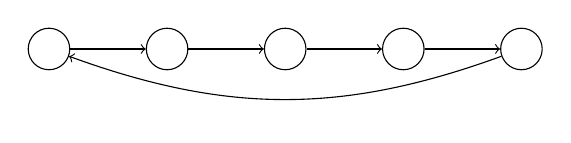
\begin{tikzpicture}
\tikzstyle{nodo} = [draw, circle, minimum size=1.5em]

\node[nodo] (A1) at (1,0) {};
\node[nodo] (A2) at (2.5,0) {};
\node[nodo] (A3) at (4,0) {};
\node[nodo] (A4) at (5.5,0) {};
\node[nodo] (A5) at (7,0) {};

\draw[->] (A1) -- (A2);
\draw[->] (A2) -- (A3);
\draw[->] (A3) -- (A4);
\draw[->] (A4) -- (A5);

\draw[->] (A5) edge [bend left=20] (A1);
\end{tikzpicture}
\caption{Anillo de procesos con $n=5$}
\label{fig:anillo}
\end{figure}

Para resolver este problema, se plantean tres comportamientos:

\begin{description}
 \item [Node] modela cada nodo del anillo.
 \item [Ring] espera un mensaje con una cantidad de nodos a crear, y una cantidad de mensajes a enviar.
 \item [BuildingRing] cumple la función de estructura de control, crea el anillo de nodos.
\end{description}

\subsubsection*{Comportamiento de Node}

\textbf{Node} reacciona entre dos comunicaciones diferentes: $'point\_to'$ y $'msg'$. En el caso de $'point\_to'$, cuando lo procesa, cambia al nodo que apunta. Cuando procesa un mensaje de tipo $['msg']$, siempre reenvía al siguiente nodo en la lista la comunicación $['msg']$. Si el valor del contador $m$ es mayor que cero, se disminuye el contador en uno y sigue con la ejecución. Si es cero, termina la ejecución en ese momento.

Código en \SAL para \textbf{Node}:

\begin{lstlisting}[language=sal, style=simple]
def Node(m, next) match
  case ['point_to', newNext]:
    become Node(m, newNext)
  case ['msg']:
    if ( m = 0 ) then
      send ['msg'] to next
    else
      send ['msg'] to next
      become Node(m - 1, next)
    end if
end def
\end{lstlisting}

Código en \CSP:

\begin{process}
Node(self, m, next) = \\ \quad
  \begin{block}
  CommRecv.self?\langle 'point\_to', newNext \rangle \then \\
  Node(self, m, newNext)
  \end{block} \\

  \Extchoice \\ \quad
  
  \begin{block}
  CommRecv.self?\langle 'msg' \rangle \then {} \\ \quad
    \begin{block}
    \If (m == 0) \Then {} \\ \quad
      \begin{block} 
      CommSend!next.\langle 'msg' \rangle \then \\
      STOP
      \end{block} \\
    \Else {} \\ \quad
      \begin{block}
      CommSend!next.\langle 'msg' \rangle \then \\
      Node(self, m - 1, next) 
      \end{block}
    \end{block}
  \end{block} 
\end{process}

% Donde:
% 
% \begin{description}
%  \item [Linea 2-3] Si responde a un mensaje de tipo $'point_to'$, el comportamiento de reemplazo es \textbf{Node} pero cambiando el parametro $next$ por $newNext$.
%  \item [Linea 4-5] Si responde a un mensaje de tipo $'msg'$, y su contador $m$ es mayor que cero, envia un mensaje al proximo actor el anillo ($next$). Su comportamiento de reemplazo es \textbf{Node} pero decrementando en uno el contador $m$.
%  \item [Linea 7] Si responde a un mensaje de tipo $'msg'$, y su contador $m$ era cero, envia un mensaje al proximo actor en el anillo ($next$). Como no define comportamiento de reemplazo, termina su ejecución en es momento.
% \end{description}

\subsubsection*{Comportamiento de Ring}

Cuando \textbf{Ring} recibe una comunicación con una lista que tiene un par de enteros, el primero de los enteros es la cantidad de nodos a crear, y el segundo es la cantidad de comunicaciones a mandar. Crea el primer nodo que va a tener el anillo y el actor que va a estar encargado de crear el resto del anillo. Le envía un mensaje a $builder$ con el número de nodos que tiene que crear. Como el primero fue inicialiado este es decrementado en uno.

Código en \SAL:

\begin{lstlisting}[language=sal, style=simple]
def Ring()[n, m]
  let first = new Node(m, nil)
      builder = new BuildingRing(first, first) 
  in
    send [n - 1, m] to builder
    become Ring() 
end def
\end{lstlisting}

Código en \CSP:

\begin{process}
Ring(self) = \\ \quad
  \begin{block}
  CommRecv.self?\langle n, m \rangle \then \\
  CreateAsk.node?first!\langle m, Null \rangle \then \\
  CreateAsk.buildingRing?builder!\langle first, first \rangle \then \\
  CommSend.builder!\langle n - 1, m\rangle \then \\
  Ring(self)
  \end{block}
\end{process}

\subsubsection*{Comportamiento de BuildingRing}

Esta es una estructura de control, siempre que procese una comunicación con $n$ mayor a uno, crea un nuevo nodo. Le envía al nodo que creó en la iteración anterior un mensaje para que apunte al nuevo nodo creado. Se auto envía un mensaje decrementando en uno el contador de nodos a crear. El comportamiento de reemplazo cambia el nodo $lastCreated$.

Si el contador $n$ era cero, le envía un mensaje al nodo creado en la iteración anterior para que apunte al primer nodo creado ($first$). De esta manera cierra el anillo. Le envía una comunicación al primer nodo, que da inicio al envío de mensajes. 

Código en \SAL:

\begin{lstlisting}[language=sal, style=simple]
def BuildingRing(m, first, lastCreated)[n, m]
  if (n == 0) then
    send ['poins_to', first] to lastCreated,
    send ['msg'] to first
  else
    let newNode = new Node(m, null) in
      send ['point_to', newNode] to lastCreated
      send [ n - 1, m ] to self
      become BuildingRing(first, newNode)
  end if
end def
\end{lstlisting}

Código en \CSP:

\begin{process}
BuildingRing(self, first, lastCreated) = \\ \quad
  \begin{block}
  CommRecv.self?\langle n, m \rangle \then \\ \quad
  \begin{block} 
  \If (n == 0) \Then {} \\ \quad
    \begin{block}
    CommSend!lastCreated.\langle 'point\_to', first \rangle \then \\
    CommSend!first.\langle 'msg' \rangle \then \\
    STOP
    \end{block} \\
  \Else {} \\ \quad
    \begin{block} 
    CreateAsk.node?newNode!\langle m, Null \rangle \then \\
    CommSend!lastCreated.\langle 'point\_to', newNode \rangle \then \\
    CommSend!self.\langle n - 1, m \rangle \then \\
    BuildingRing(self, first, newNode) 
    \end{block} \\
  \end{block} 
\end{block}
\end{process}

\section{Una semántica en CSP}

En esta sección se describen cómo traducir las expresiones, los comandos y los comportamientos desde \SAL a \CSP. Para esto se utiliza la gramática definida en \ref{actores:sal}. Las funciones esta definidas de manera inductiva.
Para notar cuando $x$ tiene la forma gramatical $H$, con la siguiente construcción: $x \equiv H$. 

\subsubsection*{Expresiones}
En la sección \ref{actores:exp} se definió la gramática para las expresiones. Para traducir estas expresiones se utilizan las siguientes funciones:
La función $exp_{tr}$ viene dada de la siguiente forma:
\begin{equation*}
  exp_{tr}(exp) =
  \setlength{\arraycolsep}{0pt}
  \renewcommand{\arraystretch}{1.2}
  \left\{\begin{array}{l @{\quad} l}
        iexp_{tr}(exp)    & \text{si $exp \equiv iexp$} \\
        bexp_{tr}(exp)    & \text{si $exp \equiv bexp$} \\
        sexp_{tr}(exp)    & \text{si $exp \equiv sexp$} \\
        idexp_{tr}(exp)   & \text{si $exp \equiv id$} \\
  \end{array}\right.
\end{equation*}

La función para las expresiones de enteros, $iexp_{tr}$, viene dada de la siguiente forma:

\begin{equation*}
\begin{array}{l c l}
iexp_{tr}(iexp_1 + iexp_2) &=& iexp_{tr}(iexp_1) + iexp_{tr}(iexp_2) \\
iexp_{tr}(iexp_1 - iexp_2) &=& iexp_{tr}(iexp_1) - iexp_{tr}(iexp_2) \\
iexp_{tr}(iexp_1 * iexp_2) &=& iexp_{tr}(iexp_1) * iexp_{tr}(iexp_2) \\ 
iexp_{tr}(iexp_1 / iexp_2) &=& iexp_{tr}(iexp_1) / iexp_{tr}(iexp_2) \\
iexp_{tr}(- iexp) &=& - iexp_{tr}(iexp) \\
iexp_{tr}(id) &=& id
\end{array}
\end{equation*}

La función expresiones booleanas, $bexp_{tr}$, es finalmente:
\begin{equation*}
\begin{array}{l c l}
bexp_{tr}(bexp_1 \textbf{ or } bexp_2) &=& bexp_{tr}(iexp_1) \vee bexp_{tr}(iexp_2) \\
bexp_{tr}(bexp_1 \textbf{ and } bexp_2) &=& bexp_{tr}(iexp_1) \wedge bexp_{tr}(iexp_2) \\
bexp_{tr}(\textbf{not } bexp) &=& \neg bexp_{tr}(bexp) \\ 
bexp_{tr}(exp_1 == iexp_2) &=& exp_{tr}(exp_1) == exp_{tr}(exp_2) \\
bexp_{tr}(id) &=& id
\end{array}
\end{equation*}

Tanto $sexp_{tr}$ como $idexp_{tr}$ no tienen una traducción asociada, podrían definirse como la función identidad.

\subsubsection*{Comportamientos}
En la sección \ref{actores:beha} se definió la gramática para los comportamientos. Para traducir estas expresiones se utilizan las funciones $beha_{tr}$ y $body_{tr}$.

La función $beha_{tr}$ viene dada por la forma:
\begin{multline*}
beha_{tr}(\textbf{def } BehName(p_1, p_2,\ldots, p_n)\ body \textbf{ end def}) = \\
BehName(self, p_1, p_2,\ldots, p_n) = body_{tr}(body) 
\end{multline*}
La función $body_{tr}$ viene dada por la forma:
\begin{multline*}
body_{tr}([ p_1, p_2,\ldots, p_n]\ command) = \\
 CommRecv.self?\langle p_1, p_2,\ldots, p_n \rangle \then cmd_{tr}(command)
\end{multline*}
\begin{multline*}
body_{tr}(\textbf{ case } [p_{11}, p_{12},\ldots, p_{1n}]: command_1 \ldots \textbf{ case } [p_{n1}, p_{n2},\ldots, p_{nk}]: command_n ) = \\
CommRecv.self?\langle p_{11}, p_{12},\ldots, p_{1n} \rangle \then cmd_{tr}(command_1) \Extchoice \ldots \Extchoice \\
CommRecv.self?\langle p_{n1}, p_{n2},\ldots, p_{nk} \rangle \then cmd_{tr}(command_n) 
\end{multline*}

\subsubsection*{Comandos}

En la sección \ref{actores:cmd} se definió la gramática para los comandos. Para traducir los comandos se utiliza la función $cmd_{tr}$, que se define de la siguiente forma:
\begin{multline*}
cmd_{tr} (\textbf{send } exp_1, exp_2, \ldots\ , exp_n \textbf{to } mexp) = \\
CommSend.mexp. \langle exp_{tr}(exp_1), exp_{tr}(exp_2), \ldots, exp_{tr}(exp_m) \rangle
\end{multline*}
\begin{multline*}
cmd_{tr} (\textbf{become}\ B(exp_1, exp_2,\ \ldots, exp_n)) = \\
B(exp_{tr}(exp_1), exp_{tr}(exp_2), \ldots, exp_{tr}(exp_n)) \rangle
\end{multline*}
\begin{multline*}
cmd_{tr} (command_1 \textbf{;} command_2) = cmd_{tr}(command_1) \then cmd_{tr}(command_2)
\end{multline*}
\begin{multline*}
cmd_{tr} (\textbf{if } bexp \textbf{ then } command_1 \textbf{ else } command_2 \textbf{ end if }) = \\
\textbf{if } (bexp_{tr}(bexp))\textbf{ then } cmd_{tr}(command_1) \textbf{ else } cmd_{tr}(command_2)
\end{multline*}
\begin{multline*}
cmd_{tr}( \textbf{let}\ id_1 = \textbf{new} B_1(exp_{11}, exp_{12},\ \ldots, exp_{1m}), \ldots, \\
id_n = \textbf{ new }B_n(exp_{n1}, exp_{n2},\ldots, exp_{nk}) \textbf{ in }command) = \\
CreateAsk.b_1?id_1! \langle exp_{tr}(exp_{11}), exp_{tr}(exp_{12}),\ \ldots, exp_{tr}(exp_{1m}) \rangle \then \ldots \\
CreateAsk.b_N?id_n! \langle exp_{tr}(exp_{n1}), exp_{tr}(exp_{n2}),\ \ldots, exp_{tr}(exp_{nk}) \rangle \then  \\ 
cmd_{tr}(command)
\end{multline*}

\subsubsection*{Pasos finales}

El sistema final consiste de todos los componentes del sistema de actores en paralelo. Los componentes a poner en paralelo son: los buzones vistos en la sección \ref{modelo:buzon}, los procesos que separan la intención de crear de la creación propiamente dicha vistos en la sección \ref{modelo:crear} y los preámbulos vistos en la misma sección.

La comunicación que va desde estos preámbulos hacia los buzones es una de las comunicaciones de interés. Los eventos en este caso son todos los generados por los buzones. Es decir el conjunto generado por $CommSend.i.j$ donde $i$ son todos los posibles actores y $j$ son los mensajes a enviar. A estos eventos se le debe unir el conjunto generado por $CommRecv.i.j$ donde $i$ son todos los posibles actores y $j$ son los mensajes a enviar. Este es el conjunto de todos los eventos posible de los buzones. Este conjunto se denomina: $Comm$.

Otra forma de comunicación a tener en cuenta es desde estos preámbulos hacia los procesos que separan la intención de crear de la creación. Es decir el conjunto generado por $CreateAsk.i.j$ donde $i$ son todos los posibles actores y $j$ son todos los posibles valores de \textit{acquaiantence-list}. A estos eventos se le debe unir el conjunto generador por $Create.i.j$ donde $i$ son todos los posibles actores y $j$ son todos los posibles valores de \textit{acquaiantence-list}. Este conjunto se denomina $Init$.

Ahora se supone que tenemos dos conjuntos de actores $ks$ y $js$, definidos de la siguiente manera:

\begin{align*}
ks = \Interleave_{ i : \{ 0 .. N\_KS \} } & Create.k?self?<p1, p2> \then K(self, p1, p2)  \\ 
js = \Interleave_{ i : \{ 0 .. N\_JS \} } & Create.j?self?<p1, p2> \then J(self, p1, p2) 
\end{align*}

donde $J$ y $K$ son dos definiciones de comportamiento. Para integrar todo el sistema de actores se escribe la siguiente ecuación:
\begin{align*}
SYSTEM =  (ks \Interleave js) \Parallel\limits_{Comm \cup Init} (Mailboxes \Interleave Creates)
\end{align*}
donde $Mailboxes$ está definido en la sección \ref{modelo:buzon} y $Creates$ en la sección \ref{modelo:crear}. Entre $ks$ y $js$ nunca existe ningún tipo de comunicación, por eso se usa el operador de entrelazado. Lo mismo ocurre con $Mailboxes$ y $Creates$.

\section{Corriendo los modelos en FDR}

Esta sección muestra algunas modificaciones necesarias que fueron hechas al modelo para poderlo correr utilizando \FDR. \FDR es un verificador de refinamiento para \CSP. Permite definir procesos de \CSP utilizando el lenguaje \CSPm. Se pueden verificar varias afirmaciones sobre estos procesos. A continuación se cuentan algunas de estas características.

\textit{probe} puede utilizarse para explorar manualmente las transiciones de un proceso como si fuera un árbol, es muy útil para al depurar una definición de proceso. Esto fue particularmente útil al explorar la creación del modelo antes propuesto. Se mostrará un caso donde se puede ver el gráfico de todas las ejecuciones de uno de los ejemplos. 
 
También es posible verificar refinamiento utilizando el modelo de trazas o el modelo divergencias. Se verá un ejemplo de como es posible verificar este tipo de afirmaciones.

Esta son algunas de las posibles pruebas que se pueden hacer utilizando la herramienta, pero no son exhaustivas. Para mayor información sobre la herramienta se puede consultar su manual\cite{fdrmanual}.

\subsection{Restricciones sobre el modelo}

Es necesario imponer restricciones al utilizar \FDR. Estas restricciones están relacionas a cómo la herramienta explora los estados posibles del modelo. Por ejemplo, si se utiliza el rango completo de enteros intentará revisar cada uno de estos enteros, haciendo cada exploración exponencial en cada estado que se visite. En el resto de esta sección se exploran estas restricciones. Las modificaciones que incluyen estas restricciones pueden verse en los ejemplos en el apéndice \ref{codigo}.

\subsubsection*{Enteros pequeños}

Para evitar la explosión de estados que causa utilizar el rango de enteros de \textit{64-bits}, se genera una una representación propia para reducirla. Para esto se utiliza un tipo algebraico que representa estos enteros:

\begin{align*}
datatype\ SmallInt =&\ SI.\{0 \ldots MAX\_INT\} | Overflow \\
\end{align*}

Donde, $MAX\_INT$ es el entero más grande que se quisiera representar. Aparte de esta representación de los enteros, se construyeron las operaciones básicas sobre ellos:

\begin{align*}
add(SI.a, SI.b)\ =&\ let\ sum\ = a + b \\
&within\ if\ sum <= MAX\_INT\ then\ SI.sum\ else\ Overflow  \\
%
sub(SI.a, SI.b) =&\ let\ sub\ =\ a - b \\
& within\ if\ sub >= 0\ then\ SI.sub\ else\ Overflow \\
%
mult(SI.a, SI.b) =&\ let\ mult\ = a * b \\
& within\ if\ mult <= MAX\_INT\ then\ SI.mult\ else\ Overflow \\
eq(SI.a, SI.b)\ =&\ a == b \\
eq(\_, \_)\ =&\ false
\end{align*}

Donde $add$ es la suma, $sub$ la resta, $mult$ la multiplicación y $eq$ la igualdad. Si alguna operación excede el entero máximo el resultado de esta es $Overflow$.

\subsubsection*{Listas de parámetros y valores}
En en modelo se utilizan listas para representar tanto los parámetros de \textit{acquaiantence-list} y los de \textit{communication-list}. Las listas son potencialmente infinitas, pare evitar que el modelo explore todos estos estados, se limita el tamaño de las listas. Se utilizan tuplas de tamaño fijo. Para esto es necesario conocer el tamaño máximo del mensaje que se va a enviar, esta es una limitación del modelo presentado.

La expresividad de los mensajes es grande. Un actor podría recibir un mensaje del tipo $['transferir', buz\acute{o}n_1, buz\acute{o}n_2]$, donde el primer buzón representa la caja de ahorro origen y el segundo la de destino. El siguiente mensaje que procese el mismo actor podría ser $['depositar', monto, buz\acute{o}n]$ donde monto es un entero con el monto a depositar y el buzón representa la caja de ahorro a la cual depositar. 

Para poder tener cierta flexibilidad en el momento de enviar mensajes, se creá una unión de tipos llamada $VALUE$. Este tipo codifica todos los posibles valores que se quisieran enviar, buzones, enteros, booleanos y cadenas. Como las tuplas se definen de tamaño fijo, es necesario agregar un tipo con la funcionalidad de marcar la posición. Esto funciona de la siguiente manera: si las listas son de tamaño tres, no necesariamente todos los mensajes son de esta longitud, podría existir un mensaje que sea una lista de tamaño dos, por ejemplo: $[1, client]$. La tupla de tamaño tres sería $(1, None, None)$. Se define $VALUE$ de la siguiente forma:

\[
  datatype\ VALUE = ACTOR.ActorID | INT.SmallInt | BOOL.Bool | ATOM.Atoms | None
\]

Las cadenas de caracteres se representa utilizando $Atoms$. Las cadenas son inmutables y la única operación que se efectúa sobre ellas es la comparación. La definición de $Atoms$ viene dada de la siguiente forma:

\[
  datatype\ Atoms = ATOM_1 | ATOM_2 | \ldots | ATOM_n
\]

\subsubsection*{Cota en el buzón}

Se puede modelar un buzón que no tenga una cota superior, pero se tendría nuevamente problemas de explosión de estados ya que \FDR intentaría explorar todas las combinaciones posibles de buzón. Este caso es similar al de la lista en la comunicación. 

La ecuación de \textit{buzón}, con cota, es la siguiente:

\begin{process}

\begin{block}
MAILBOX\_SIZE = 4
\end{block} \\

\begin{block}
Mailbox(i, \nil) = {} \\ \quad
CommSend?i.x \then Mailbox(i, \lseq x \rseq) 
\end{block} \\

\begin{block}
Mailbox(i, msgs) = {} \\ \quad
  \begin{block} 
  \If (length(msgs) < MAILBOX\_SIZE - 1) \Then {} \\ \quad
    \begin{block} 
      MailboxWithSpace(i, msgs)
    \end{block} \\
  \Else {} \\ \quad
    \begin{block}
      MailboxFull(i, msgs)
    \end{block}
  \end{block} 
\end{block} \\

\begin{block}
MailboxWithSpace(i, \lseq x \rseq \cat xs ) = {} \\ \quad 
  \begin{block}
    CommRecv!i.x \then Mailbox(i, xs) \\
    \Extchoice \\
    CommSend?i.y \then Mailbox(i, \lseq x \rseq \cat xs \cat \lseq y \rseq ) 
  \end{block}
\end{block} \\

\begin{block}
MailboxFull(i, \lseq x \rseq \cat xs ) = {} \\ \quad 
  \begin{block}
    CommRecv!i.x \then Mailbox(i, xs) \\
  \end{block}
\end{block} \\
\end{process}

La ecuación anterior le agrega a la vista en la sección \ref{modelo:buzon}, un límite definido por $MAILBOX\_SIZE$. El comportamiento del proceso buzón depende de su estado, si no tiene ningún mensaje, o si tiene al menos algún mensaje o si está completo.

\begin{itemize}
\item Si no tiene ningún mensaje, solo sincroniza mensajes por el canal $CommSend$.
\item Si tiene algunos mensajes, por los canales $CommSend$ y $CommRecv$.
\item Si llegó a su capacidad máxima $MAILBOX\_SIZE$ lo hace solo por el canal $CommRecv$.
\end{itemize}

\subsection{Algunos resultados}

A continuación se muestran dos resultados obtenidos utilizando el modelo propuesto en \CSP. Uno explora el gráfico de entrelazado y el otro verifica una afirmación utilizando el modelo de trazas.

\subsubsection*{Gráfico de interacciones}

Utilizando la función \textit{probe} en herramienta \FDR, se puede ver permite ver gráfico de interacciones de los distintos procesos. En el caso del modelo, permite ver como las diferentes interacciones de los actores.

\begin{figure}[H]

\begin{center}
\includegraphics[width=15 cm]{img/fact.png}
\caption{Calculo del factorial de 3 visto en \ref{fig:factorial}}\label{modelo:grafo}
\end{center}
\end{figure}

Se pueden ver en la figura \ref{modelo:grafo} las siguientes acciones:

\begin{itemize}
\item $Main$ crea un actor con el comportamiento $Factorial$
\item $Main$ le envía a $Factorial$, un mensaje con su dirección de buzón y el número 3.
\item Se crea el actor $Factorial$
\item $Factorial$ recibe el mensaje con la dirección de $Main$ y el número 3.

\item $Factorial$ crea un actor de tipo $FactorialWorker$ ($factorialWorker_1$). Está inicializado con los parámetros: el entero 3, y el buzón del actor $Main$.
\item $Factorial$ se auto envía el mensaje con el valor 2 y la dirección de buzón de $factorialWorker_1$.
\item $Factorial$ recibe el mensaje con la dirección de $factorialWorker_1$ y el número 2.
\item Se crea el actor $FactorialWorker$ con buzón $factorialWorker_1$.

\item $Factorial$ crea un actor de tipo $FactorialWorker$ ($factorialWorker_2$). Está inicializado con los parámetros: el entero 3, y el buzón del actor $factorialWorker_1$.
\item $Factorial$ se auto envía el mensaje con el valor 1 y la dirección de buzón de $factorialWorker_2$.
\item $Factorial$ recibe el mensaje con la dirección de $factorialWorker_2$ y el número 1.
\item Se crea el actor $FactorialWorker$ con buzón $factorialWorker_2$.

\item $Factorial$ crea un actor de tipo $FactorialWorker$ ($factorialWorker_3$). Está inicializado con los parámetros: el entero 1, y el buzón del actor $factorialWorker_2$.
\item $Factorial$ se auto envía el mensaje con el valor 0 y la dirección de buzón de $factorialWorker_3$.
\item $Factorial$ recibe el mensaje con la dirección de $factorialWorker_3$ y el número 0.
\item Se crea el actor $FactorialWorker$ con buzón $factorialWorker_3$.

\item $Factorial$ le envía a $factorialWorker_3$ el entero 1.
\item $factorialWorker_3$ recibe el valor 1.

\item $factorialWorker_3$ le envía a $factorialWorker_2$ el entero 1.
\item $factorialWorker_2$ recibe el valor 1.

\item $factorialWorker_2$ le envía a $factorialWorker_1$ el entero 2.
\item $factorialWorker_1$ recibe el valor 2.

\item $factorialWorker_1$ le envía a $Main$ el entero 6.
\item $Main$ recibe el valor 6.

\end{itemize}

Esta captura fue realizada utilizando el comando \verb=:probe SYSTEM= en \FDR en el código de factorial del apéndice \ref{codigo:factorial}.

\subsubsection*{Refinamiento}

En \FDR para probar si un proceso P refina en un proceso Q se escribe \verb$assert P [T= Q$. Para hacer una prueba de refinamiento se utiliza el ejemplo de la cola visto en la sección \ref{ejemplo:cola}. El código en \CSPm de este se encuentra en el apéndice \ref{codigo:cola}. El mismo cuenta con dos actores ``main'', \verb=actor_main1= y \verb=actor_main2=, donde:

El actor \verb=actor_main1=, después de crear un actor \textit{Queue}, hace uso de la selección externa para:
\begin{itemize}
 \item enviar a el actor \textit{Queue} un mensaje $['enqueue', 1]$
 \item enviar a el actor \textit{Queue} un mensaje $['enqueue', 2]$
 \item enviar a el actor \textit{Queue} un mensaje $['dequeue', buzonDeMain]$, seguido de esperar recibir un entero.
\end{itemize}

El actor \verb=actor_main2=, después de crear un actor \textit{Queue}, hace uso de la selección externa para:
\begin{itemize}
 \item enviar a el actor \textit{Queue} un mensaje $['enqueue', 1]$, seguido de enviar a el actor \textit{Queue} un mensaje $['enqueue', 2]$
 \item enviar a el actor \textit{Queue} un mensaje $['dequeue', buzonDeMain]$, seguido de esperar recibir un entero.
\end{itemize}

El resultado de poner en paralelo todos los componentes del sistema utilizando \verb=actor_main1= se llama \verb=SYSTEM1=. En el caso de \verb=actor_main2= se llama \verb=SYSTEM2=. Esto puede verse en el código de \CSPm.

\begin{figure}[H]
\begin{center}
\includegraphics[width=5 cm]{img/trazas.png}
\caption{Resultado de las afirmaciones}\label{modelo:verifica}
\end{center}
\end{figure}

Para probar si $SYSTEM1$, refina en $SYSTEM2$ se utiliza la siguiente afirmación: \verb$assert SYSTEM1 [T= SYSTEM2$. Para probar si $SYSTEM2$, refina en $SYSTEM1$ se utiliza la siguiente afirmación: \verb$assert SYSTEM2 [T= SYSTEM1$.

Puede verse en la figura \ref{modelo:verifica} el resultado de correr ambas afirmaciones. Utilizando la herramienta se encuentra un contraejemplo donde $SYSTEM2$ no refina en $SYSTEM1$ como muestra la figura \ref{modelo:contraejemplo}.

La intuición detrás de por que $SYSTEM1$ refina en $SYSTEM2$, y que $SYSTEM2$ no refina en $SYSTEM1$ tiene que ver con que $SYSTEM1$ es menos restrictivo que $SYSTEM2$. El actor \verb=actor_main1= puede elegir entre entre dos opciones para desencolar, y el actor \verb=actor_main2= solo una y con un orden preestablecido.

\begin{figure}[H]
\begin{center}
\includegraphics[width=15 cm]{img/contraejemplo.png}
\caption{Contraejemplo de SYSTEM2 no refina en SYSTEM1}\label{modelo:contraejemplo}
\end{center}
\end{figure}
 
 % Modelo en CSP

\chapter{Formaliznado la semantica en CSP}

TODO: Definir \textbf{translateExp}

La clase \textbf{Cmnd} con elementos de tipo S está dada por:

\begin{verbatim}
S :== S_1 ; S_2 | if b then S_1 else S_2 | send [e1, .., e_i] to a | become new
E(e_1, .. ,e_i) | let a_1 = new E_1(e_1,..,e_i) and ... a_j = new
E_1(e_1,..,e_i) { S } 
\end{verbatim}

definimos la funcion \textbf{translateCmd} de la siguiente forma:

\begin{verbatim}
translateCmd (S_1 S_2) = translateCmd(S_1) -> translateCmd(S_2)
\end{verbatim}


\begin{verbatim}
translateCmd(if b then S_1 else S_2) = 
   if (translateExp(b)) then
       translateCmd(S_1) else 
       translateCmd(S_2)
\end{verbatim}

\begin{verbatim}
translateCmd(send[e_1, ..., e_i] to a) = CommSend.a.
         (translateExp(e_1), ..., 
          translateExp(e_i)) 
\end{verbatim}

\begin{verbatim}
translateCmd(become new Beh(e_1, ..., e_n)) = runningBeh(self, e_1, ..., e_n)
\end{verbatim}

newEnv es el resultado de agregar a el entorno de las variables de mailbox $a_1
= E_1.pid_1$ .. $a_n = E_n.pid_n$
\begin{verbatim}
translateCmd(let a_1 = new E_1(e_1, ..., e_j) and 
         ... and a_n = new E_N(e_1, ..., e_j) { S } = 

CreateAsk?E_1.pid_1!(translateExp(e_1), ...,translateExp(e_j)) ->
CreateAsk?E_N.pid_n!(translateExp(e_1), ...,translateExp(e_j)) ->
translateCmd(S, newEnv)
\end{verbatim}


La clase \textbf{Beha} con elementos de tipo S está dada por:

\begin{verbatim}
def behName(a_1 .. a_i)[n_1 ... n_j]
  S
end def
\end{verbatim}

Tendria como equivalente en CSP:

\begin{verbatim}

behName = ||| actorId : {|BehName|} @ Create.actorId?(a_1, ..., a_i) ->
behNameRunning(actorId, a_1, .., a_n)

behNameRunning(self, a_1, .., a_n) = CommRecv.self(n_1 ... n_j) -> translateCmd(S)

\end{verbatim}
 % Formalización

% \chapter{Conclusiones}

La primera motivación de este trabajo consistió comprender los elementos básicos del modelo de actores. En segunda instancia fue generar un modelo en \CSP, y hacer con este algunas pruebas en \FDR. Fue interesante explorar los distintos mecanismos de paralelismo que tiene \CSP a la hora de componer procesos. 

El mayor esfuerzo involucrado tiene que ver con lograr que el modelo de actores corriera en \FDR, de ahí vienen las restricciones enunciadas en el capítulo anterior. Sin dudar el aporte de \FDR permitió entender que el modelo realmente funcionaba. Fue interesante poder observar el árbol de ejecución utilizando el comando \verb=probe= de \FDR. 

El trabajo original de Agha\cite{Agha:1986:AMC:7929}, modelaba los mensajes como una 3-tupla. Además del actor destino y el mensaje este agregaba un \textit{TAG} que después utilizaba en el modelo denotacional que construyó para prefijar la creación de las nuevas direcciones de buzón. Este claramente no es un problema trivial de resolver, en el caso del presente trabajo varios modelos se probaron hasta llegar el propuesto en la sección \ref{modelo:crear}. El momento de creación y el paso inicial de mensajes es uno de los puntos fuertes del modelo de actores.

Otro de los puntos más interesantes a resaltar del modelo, es la conclusión de que todo la fuerza que impulsa el modelo son los mensajes sin procesar. Este concepto es fundamental para cualquier trabajo relacionado con la exploración del grafo de entrelazado, ya que los actores son deterministas, recorrer este grafo está relacionado con el orden en el que se procesan estos mensajes.

La expresividad entorno a la construcción del mensaje como tal, hace muy compleja la tarea de fijar una restriccion sobre los tipos de datos que se fueran a comunicar de un actor a otro.

El modelo de buzón que se utilizó tiene solo disponible para ser consumido el mensaje que está primero en el buzón. Se podría usar el presente modelo para analizar las diferencias con el modelo en el cual todos los mensajes que están dentro del buzón están disponibles para ser consumidos.
 % Conclusiones 


\bibliography{references}{}
\bibliographystyle{plain}

\end{document}


